% talk_v6.tex — SHiP Timing Bar: Definitive Scientific Presentation
% Author: René Ríos / Universidad de La Serena (ULS)
% Compiled: pdflatex (WSL2, TeX Live 2020)
% Philosophy: Napkin first. Geant4 second.

\documentclass[aspectratio=169,9pt]{beamer}
\usetheme{Warsaw}
\usecolortheme{seahorse}
\setbeamertemplate{headline}{}
\setbeamertemplate{navigation symbols}{}
\setbeamertemplate{footline}[frame number]

\usepackage{amsmath,amssymb}
\usepackage{booktabs,tabularx,colortbl}
\usepackage{graphicx}
\usepackage{tikz}
\usetikzlibrary{arrows.meta,decorations.pathreplacing,patterns,calc,shapes.geometric}

% ---- convenience macros ----
\newcommand{\anafig}[1]{\includegraphics[width=\linewidth]{figs/#1}}
\newcommand{\ps}{\,\text{ps}}
\newcommand{\mm}{\,\text{mm}}
\newcommand{\ns}{\,\text{ns}}

% ---- napkin numbers (from napkin_macros.tex) ----
\newcommand{\thetac}{39.27^{\circ}}
\newcommand{\fTIR}{0.548}
\newcommand{\fTIRend}{0.274}
\newcommand{\vgroup}{189.7\mm/\text{ns}}
\newcommand{\Nbounce}{85.6}
\newcommand{\NbounceW}{14.3}
\newcommand{\LambdaH}{405\mm}
\newcommand{\Rvikuiti}{0.95}
\newcommand{\NpeNapkin}{570}
\newcommand{\NpeG}{701.3}
\newcommand{\sigmaENDval}{53.68\ps}
\newcommand{\sigmaTOPval}{15.20\ps}
\newcommand{\sigmaBLUEval}{15.21\ps}
% EXEC_23 FIX-03: w_END not resolved at n=5000 (CP-B wscan); kept for G1 formula display only
\newcommand{\wEND}{0.013}  % one convention (best_est mixed); not canonical
\newcommand{\wTOP}{0.987}  % correspondingly; not canonical
\newcommand{\veffEND}{177.6\mm/\text{ns}}
\newcommand{\sigmax}{7.9\mm}
% EXEC_24 FIX-11: bare-number macros for G1 formula and G2 table
\newcommand{\sigmaENDbval}{53.68}      % bare σ_E (ps); hybrid m=8 x=0
\newcommand{\sigmaTOPbval}{15.20}      % bare σ_T (ps); k=3 x=0
\newcommand{\CETval}{196.3}            % C_ET best_est and empirical (ps²)
\newcommand{\CETrobust}{80.5}          % C_ET robust IQR polarization (ps²)
\newcommand{\wENDrobust}{0.051}        % w_E robust IQR; not canonical
\newcommand{\wENDemp}{0.086}           % w_E empirical np.var+np.cov; not canonical
\newcommand{\sigBLUEbestest}{15.21}    % σ_IQR^ev best_est (ps, bare)
\newcommand{\sigBLUErobust}{15.12}     % σ_IQR^ev robust IQR (ps, bare)
\newcommand{\sigBLUEemp}{15.03}        % σ_IQR^ev empirical (ps, bare)
\newcommand{\sigmaformBLUE}{15.18}     % σ^formula Gaussian BLUE algebra (ps, bare)
% w* from CP-B wscan (biased argmin, not a reported result)
\newcommand{\wstarxzero}{0.080}        % w*(x=0); blue_wscan_x0.meta.json
\newcommand{\wstarxptwo}{0.125}        % w*(x=+200); ρ(x) check
\newcommand{\wstarxpsix}{0.065}        % w*(x=+600); ρ(x) check
% σ_TOP at off-center positions (G2 qualitative check)
\newcommand{\sigmaTOPxptwo}{24.3}      % bare σ_TOP (ps) at x=+200
\newcommand{\sigmaTOPxpsix}{16.8}      % bare σ_TOP (ps) at x=+600

% ---- auto-generated macro files ----
% napkin_macros.tex — AUTO-GENERATED by napkin.py, do not edit

\newcommand{\Napnpvt}{1.580}  % PVT refractive index
\newcommand{\Napthetacdeg}{39.27\,\text{deg}}  % Critical angle: arcsin(1/n)
\newcommand{\NapfTIR}{0.5484}  % TIR fraction (slab): 2cos(θ_c)−1  [Knoll 8.15]
\newcommand{\NapfTIRperend}{0.2742}  % TIR fraction toward one end: f_TIR/2
\newcommand{\Napvgroupmmns}{189.7\,\text{mm/ns}}  % Group velocity: c/n
\newcommand{\NapdEMeV}{2.000\,\text{MeV}}  % Energy deposited: 1-GeV μ⁻ through H=10 mm
\newcommand{\NapRvikuiti}{0.9500}  % Vikuiti non-TIR reflectivity (Materials.cc)
\newcommand{\NapNbounce}{35.00}  % Bounces to traverse L/2 along H-faces
\newcommand{\NapRsurvbounce}{0.1661}  % Vikuiti bounce survival: R^N_bounce
\newcommand{\NapdEdxMeVcm}{2.000\,\text{MeV/cm}}  % MIP dE/dx in PVT (minimum ionising)
\newcommand{\NapLmm}{1400\,\text{mm}}  % Bar length
\newcommand{\NapWmm}{60.00\,\text{mm}}  % Bar width
\newcommand{\NapHmm}{10.00\,\text{mm}}  % Bar height (thin direction)
\newcommand{\Napnsipmperend}{8.000}  % SiPM per END face
\newcommand{\NapyieldejA}{10000\,\text{ph/MeV}}  % EJ-200 scintillation yield
\newcommand{\NaptauriseejA}{0.9000\,\text{ns}}  % EJ-200 rise time
\newcommand{\NaptaudecayejA}{2.100\,\text{ns}}  % EJ-200 decay time
\newcommand{\NaplattmmejA}{3800\,\text{mm}}  % EJ-200 attenuation length (mm)
\newcommand{\NaplattcmejA}{380.0\,\text{cm}}  % EJ-200 attenuation length (cm)
\newcommand{\NapbulksurvejA}{0.8318}  % EJ-200 bulk survival: exp(−700/3800)
\newcommand{\NapNprodejA}{20000\,\text{photons}}  % EJ-200 photons produced: yield×dE
\newcommand{\NapNpesimejA}{1311\,\text{pe}}  % EJ-200 simulated Npe/end at x=0
\newcommand{\NapfeffejA}{0.0655}  % EJ-200 collection×PDE: Npe_sim/N_produced
\newcommand{\NapsigmasimejA}{47.60\,\text{ps}}  % EJ-200 simulated σ(T0) at x=0
\newcommand{\NapsigmaxejA}{6.386\,\text{mm}}  % EJ-200 position resolution: σ·v_g/√2
\newcommand{\NapyieldejB}{10400\,\text{ph/MeV}}  % EJ-204 scintillation yield
\newcommand{\NaptauriseejB}{0.7000\,\text{ns}}  % EJ-204 rise time
\newcommand{\NaptaudecayejB}{1.800\,\text{ns}}  % EJ-204 decay time
\newcommand{\NaplattmmejB}{1600\,\text{mm}}  % EJ-204 attenuation length (mm)
\newcommand{\NaplattcmejB}{160.0\,\text{cm}}  % EJ-204 attenuation length (cm)
\newcommand{\NapbulksurvejB}{0.6456}  % EJ-204 bulk survival: exp(−700/1600)
\newcommand{\NapNprodejB}{20800\,\text{photons}}  % EJ-204 photons produced: yield×dE
\newcommand{\NapNpesimejB}{941.0\,\text{pe}}  % EJ-204 simulated Npe/end at x=0
\newcommand{\NapfeffejB}{0.0452}  % EJ-204 collection×PDE: Npe_sim/N_produced
\newcommand{\NapsigmasimejB}{52.10\,\text{ps}}  % EJ-204 simulated σ(T0) at x=0
\newcommand{\NapsigmaxejB}{6.990\,\text{mm}}  % EJ-204 position resolution: σ·v_g/√2
\newcommand{\NapyieldejC}{9700\,\text{ph/MeV}}  % EJ-230 scintillation yield
\newcommand{\NaptauriseejC}{0.5000\,\text{ns}}  % EJ-230 rise time
\newcommand{\NaptaudecayejC}{1.500\,\text{ns}}  % EJ-230 decay time
\newcommand{\NaplattmmejC}{1200\,\text{mm}}  % EJ-230 attenuation length (mm)
\newcommand{\NaplattcmejC}{120.0\,\text{cm}}  % EJ-230 attenuation length (cm)
\newcommand{\NapbulksurvejC}{0.5580}  % EJ-230 bulk survival: exp(−700/1200)
\newcommand{\NapNprodejC}{19400\,\text{photons}}  % EJ-230 photons produced: yield×dE
\newcommand{\NapNpesimejC}{701.3\,\text{pe}}  % EJ-230 simulated Npe/end at x=0
\newcommand{\NapfeffejC}{0.0361}  % EJ-230 collection×PDE: Npe_sim/N_produced
\newcommand{\NapsigmasimejC}{49.60\,\text{ps}}  % EJ-230 simulated σ(T0) at x=0
\newcommand{\NapsigmaxejC}{6.655\,\text{mm}}  % EJ-230 position resolution: σ·v_g/√2
\newcommand{\NapratiopredejB}{0.8073}  % EJ-204/EJ-200 Npe ratio (napkin prediction)
\newcommand{\NapratioobsejB}{0.7179}  % EJ-204/EJ-200 Npe ratio (simulation)
\newcommand{\NapratiopredejC}{0.6508}  % EJ-230/EJ-200 Npe ratio (napkin prediction)
\newcommand{\NapratioobsejC}{0.5350}  % EJ-230/EJ-200 Npe ratio (simulation)
\newcommand{\Napveffendmmns}{184.6\,\text{mm/ns}}  % Effective propagation velocity (END, EJ-230)
\newcommand{\NapsigmaDtendps}{111.5\,\text{ps}}  % σ of (t_R−t_L) for END estimator
\newcommand{\Napsigmaxendmm}{10.29\,\text{mm}}  % Position resolution: (veff/2)·σΔt
\newcommand{\Napbetaeffenddeg}{13.37\,\text{deg}}  % Effective axial angle END: arccos(veff/vg)
\newcommand{\Napalphacdeg}{50.73\,\text{deg}}  % Angle from bar surface for ray just outside TIR
\newcommand{\Naptanalphac}{1.223}  % tan(α_c) for bounce counting formula
\newcommand{\NapNbounceH}{85.63}  % Bounces on H=10 mm face to reach L/2
\newcommand{\NapNbounceW}{14.27}  % Bounces on W=60 mm face to reach L/2
\newcommand{\NapRviknap}{0.9800}  % Vikuiti reflectivity (napkin, manufacturer spec)
\newcommand{\NapLambdareflHmm}{404.6\,\text{mm}}  % Reflector attenuation length, H=10 mm face
\newcommand{\NapLambdareflWmm}{2428\,\text{mm}}  % Reflector attenuation length, W=60 mm face
\newcommand{\Napsipmactivemmsq}{288.0\,\text{mm2}}  % Total SiPM active area per END face (8×36)
\newcommand{\Napendfacemmsq}{600.0\,\text{mm2}}  % END face area: W×H = 60×10
\newcommand{\Napfcoverage}{0.4800}  % SiPM coverage fraction: 288/600
\newcommand{\NapPDEnapkin}{0.4000}  % Assumed PDE for napkin budget
\newcommand{\NapNtirendC}{5320\,\text{photons}}  % EJ-230: TIR-guided toward one end
\newcommand{\NapNbulksurvC}{2969\,\text{photons}}  % EJ-230: after bulk attenuation (70 cm)
\newcommand{\NapNatsipmC}{1425\,\text{photons}}  % EJ-230: reaching SiPM surface
\newcommand{\NapNpenapkinC}{570.0\,\text{pe}}  % EJ-230: napkin Npe/end (TIR-only path)
\newcommand{\NapNpeLRC}{1140\,\text{pe}}  % EJ-230: napkin Npe L+R total
\newcommand{\Napfescapecone}{0.1129}  % Escape cone fraction at END: (1−cosθ_c)/2
\newcommand{\Napnpeidxmatch}{570.0\,\text{pe}}  % EJ-230 napkin Npe/end (index-matched coupling)
\newcommand{\Napnpeairgap}{234.6\,\text{pe}}  % EJ-230 napkin Npe/end (air-gap escape cone only)
\newcommand{\NapratiovikTIRhi}{2.429}  % Napkin max Vikuiti/TIR ratio (air-gap case ≈ 2.4)
\newcommand{\NapsigmaENDbestps}{53.68\,\text{ps}}  % Best σ_END (m*=8): EJ-230 + Vikuiti, x=0
\newcommand{\NapsigmaTOPbestps}{15.20\,\text{ps}}  % Best σ_TOP (k*=3): EJ-230 + 20 TOP SiPMs
\newcommand{\NapsigmaBLUEbestps}{15.21\,\text{ps}}  % Best σ_BLUE: BLUE combination at x=0
\newcommand{\NapwTOPbest}{0.9870}  % BLUE weight for TOP estimator
\newcommand{\NapwENDbest}{0.0130}  % BLUE weight for END estimator

% results_macros.tex — AUTO-GENERATED by scripts/results_macros.py, do not edit
% Source: analysis/optim/phase_ab_optimal.csv

% EJ-200
\newcommand{\RessigmaxzEROejA}{54.86\,\text{ps}}  % EJ-200 sigma_m*(x=0) with units
\newcommand{\RessigmabxzEROejA}{54.86}  % EJ-200 sigma_m*(x=0) bare (for table)
\newcommand{\ResmoptxzEROejA}{5}  % EJ-200 m* at x=0
\newcommand{\RessigmamEANejA}{52.72\,\text{ps}}  % EJ-200 bar-mean sigma_m* with units
\newcommand{\RessigmabmEANejA}{52.72}  % EJ-200 bar-mean sigma_m* bare (for table)
\newcommand{\RessigmaMINejA}{47.57\,\text{ps}}  % EJ-200 min sigma_m* on bar
\newcommand{\ResxMINejA}{-600\,\text{mm}}  % EJ-200 x at min sigma
\newcommand{\ResNpexzEROejA}{1311\,\text{pe}}  % EJ-200 mean N_pe/end at x=0

% EJ-204
\newcommand{\RessigmaxzEROejB}{53.36\,\text{ps}}  % EJ-204 sigma_m*(x=0) with units
\newcommand{\RessigmabxzEROejB}{53.36}  % EJ-204 sigma_m*(x=0) bare (for table)
\newcommand{\ResmoptxzEROejB}{10}  % EJ-204 m* at x=0
\newcommand{\RessigmamEANejB}{53.57\,\text{ps}}  % EJ-204 bar-mean sigma_m* with units
\newcommand{\RessigmabmEANejB}{53.57}  % EJ-204 bar-mean sigma_m* bare (for table)
\newcommand{\RessigmaMINejB}{52.07\,\text{ps}}  % EJ-204 min sigma_m* on bar
\newcommand{\ResxMINejB}{-300\,\text{mm}}  % EJ-204 x at min sigma
\newcommand{\ResNpexzEROejB}{941\,\text{pe}}  % EJ-204 mean N_pe/end at x=0

% EJ-230
\newcommand{\RessigmaxzEROejC}{50.49\,\text{ps}}  % EJ-230 sigma_m*(x=0) with units
\newcommand{\RessigmabxzEROejC}{50.49}  % EJ-230 sigma_m*(x=0) bare (for table)
\newcommand{\ResmoptxzEROejC}{7}  % EJ-230 m* at x=0
\newcommand{\RessigmamEANejC}{51.95\,\text{ps}}  % EJ-230 bar-mean sigma_m* with units
\newcommand{\RessigmabmEANejC}{51.95}  % EJ-230 bar-mean sigma_m* bare (for table)
\newcommand{\RessigmaMINejC}{49.55\,\text{ps}}  % EJ-230 min sigma_m* on bar
\newcommand{\ResxMINejC}{+100\,\text{mm}}  % EJ-230 x at min sigma
\newcommand{\ResNpexzEROejC}{701\,\text{pe}}  % EJ-230 mean N_pe/end at x=0

% ---- derived aliases ----
\newcommand{\sigmaENDonlyval}{\RessigmaxzEROejC}   % EJ-230 END-only m*=7 x=0, phase_ab_optimal.csv

% ---- colors ----
\definecolor{colEND}{RGB}{0,102,178}
\definecolor{colTOP}{RGB}{204,102,0}
\definecolor{colBLUE}{RGB}{0,153,76}
\definecolor{colOracle}{RGB}{120,120,120}
\definecolor{colNap}{RGB}{178,0,102}

% ====================================================================
\title[SHiP Timing Bar]{SHiP Timing Bar:\\From First Principles to Precision Timing}
\subtitle{EJ-230 + Vikuiti ESR | Napkin First, Geant4 Second}
\author[René Ríos (ULS)]{René Ríos\\[2pt]
  \small Universidad de La Serena (ULS)}
\date{August 2026}
% ====================================================================

\begin{document}

\begin{frame}
  \titlepage
\end{frame}

\begin{frame}{Outline}
  \tableofcontents[hideallsubsections]
\end{frame}

% ====================================================================
\section{Optical Physics (First Principles)}
% ====================================================================

\begin{frame}{The Bar and the Physics Problem}
  \begin{columns}[T]
    \column{0.52\linewidth}
    \textbf{SHiP timing layer:} reject scattered muon background from charm/tau decays.
    Target: $\sigma_t < 100\ps$.\\[1pt]
    {\footnotesize $t_0$ = instant of muon–bar interaction (``clock start'');
    $\sigma_t = \sigma(\hat{t}_0 - t_0)$, reconstructed from SiPM hit times.}\\[4pt]
    \textbf{The detector bar:} $1400\times 60\times 10\,\text{mm}^3$ EJ-230 scintillator.\\[4pt]
    \textbf{Readout:} END SiPMs (8 per face) + TOP SiPMs ($N_\text{TOP}$ along the bar).\\[4pt]
    \textbf{Reflector:} Vikuiti ESR on all non-SiPM surfaces ($R = \Rvikuiti$).\\[5pt]
    \begin{block}{\footnotesize What is the ``napkin''?}
      \footnotesize
      A first-principles back-of-envelope estimate using the bar geometry
      and the optical physics of TIR in a slab (Knoll, Ch.~8).
      It predicts trends analytically.
      Geant4 then confirms or reveals corrections.
    \end{block}

    \column{0.44\linewidth}
    % Bar geometry TikZ
    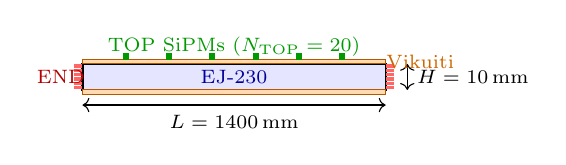
\begin{tikzpicture}[scale=0.55, every node/.style={font=\scriptsize}]
      % Main bar
      \fill[blue!10] (0,0) rectangle (7,0.6);
      \draw[thick] (0,0) rectangle (7,0.6);
      % Vikuiti top/bottom
      \fill[orange!30] (0,0.6) rectangle (7,0.7);
      \fill[orange!30] (0,-0.1) rectangle (7,0);
      \draw[orange!70!black] (0,0.6) rectangle (7,0.7) node[right, xshift=1pt] {};
      \draw[orange!70!black] (0,-0.1) rectangle (7,0) {};
      % END SiPMs left
      \foreach \y in {0.05,0.15,0.25,0.35,0.45,0.55} {
        \fill[red!60] (-0.2,\y-0.04) rectangle (0,\y+0.04);
      }
      % END SiPMs right
      \foreach \y in {0.05,0.15,0.25,0.35,0.45,0.55} {
        \fill[red!60] (7,\y-0.04) rectangle (7.2,\y+0.04);
      }
      % TOP SiPMs
      \foreach \x in {1,2,3,4,5,6} {
        \fill[green!60!black] (\x-0.07,0.7) rectangle (\x+0.07,0.85);
      }
      % Dimensions
      \draw[<->] (0,-0.35) -- (7,-0.35) node[midway,below] {$L=1400\mm$};
      \draw[<->] (7.5,0) -- (7.5,0.6) node[midway,right] {$H=10\mm$};
      % Labels
      \node[red!70!black] at (-0.5,0.3) {END};
      \node[green!60!black] at (3.5,1.0) {TOP SiPMs ($N_\text{TOP}=20$)};
      \node[orange!70!black] at (3.5,-0.25) {};
      \node[orange!80!black,font=\scriptsize] at (7.8,0.65) {Vikuiti};
      \node[blue!60!black] at (3.5,0.3) {EJ-230};
    \end{tikzpicture}\\[2pt]
    \footnotesize $W=60\mm$; $8$ END SiPMs per face ($6\times6\,\text{mm}^2$).
  \end{columns}
\end{frame}

% ---- TIR ----
\begin{frame}{Total Internal Reflection Channels Photons to the Ends}
  \begin{columns}[T]
    \column{0.48\linewidth}
    For EJ-230 ($n = 1.58$, air $n_0 = 1$):\\[4pt]
    \[
      \theta_c = \arcsin\!\left(\tfrac{1}{1.58}\right) = \thetac
    \]
    \textbf{TIR fraction} (slab geometry, Knoll Ch.~8 §III):
    \[
      f_\text{TIR} \approx 2\cos\theta_c - 1 = \fTIR
    \]
    Photons hitting the $H=10\mm$ face at $\theta>\theta_c$ from the normal
    are totally reflected and guided toward the ends.\\[3pt]
    \textbf{Per end} (half travel rightward):
    \[
      f_\text{TIR/end} = \tfrac{f_\text{TIR}}{2} = \fTIRend
    \]
    \alert{54.8\% of photons are TIR-trapped.}\\[3pt]
    The remaining 45.2\% escape through the $H$-faces
    but are recovered by the Vikuiti reflector (Population II).

    \column{0.48\linewidth}
    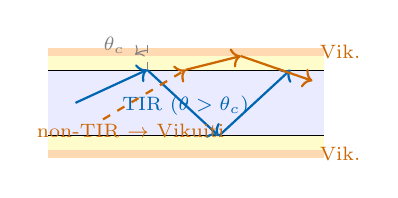
\begin{tikzpicture}[scale=0.70, every node/.style={font=\scriptsize}]
      % Bar cross-section (H direction)
      \fill[blue!8] (0,0) rectangle (5,1.2);
      \draw[thick] (0,0) -- (5,0);
      \draw[thick] (0,1.2) -- (5,1.2);
      % Air + Vikuiti top
      \fill[yellow!20] (0,1.2) rectangle (5,1.45);
      \fill[orange!30] (0,1.45) rectangle (5,1.6);
      % Air + Vikuiti bottom
      \fill[yellow!20] (0,-0.25) rectangle (5,0);
      \fill[orange!30] (0,-0.4) rectangle (5,-0.25);
      % TIR ray (steep, bounces)
      \draw[->,colEND,thick] (0.5,0.6) -- (1.8,1.2);
      \draw[->,colEND,thick] (1.8,1.2) -- (3.1,0);
      \draw[->,colEND,thick] (3.1,0) -- (4.4,1.2);
      \node[colEND] at (2.5,0.55) {TIR ($\theta>\theta_c$)};
      % Escape ray (shallow)
      \draw[->,colTOP,thick,dashed] (1.0,0.3) -- (2.5,1.2);
      \draw[->,colTOP,thick] (2.5,1.2) -- (3.5,1.45);
      \draw[->,colTOP,thick] (3.5,1.45) -- (4.8,1.0);
      \node[colTOP] at (1.5,0.1) {non-TIR $\to$ Vikuiti};
      % Angle label
      \draw[dashed,gray] (1.8,1.2) -- (1.8,1.7);
      \draw[->,gray] (1.8,1.55) arc[start angle=90,end angle=128,radius=0.35];
      \node[gray] at (1.2,1.65) {$\theta_c$};
      % Labels
      \node[orange!80!black] at (5.3,1.52) {Vik.};
      \node[orange!80!black] at (5.3,-0.32) {Vik.};
    \end{tikzpicture}
    \vspace{2pt}\\
    \footnotesize\textit{Blue}: TIR-guided (54.8\%); \textit{orange dashed}: non-TIR, recovered by reflector.
  \end{columns}
\end{frame}

% ---- Two populations ----
\begin{frame}{Two Photon Populations Drive the Timing}
  \begin{columns}[T]
    \column{0.48\linewidth}
    \textbf{Population I: TIR-guided}
    \begin{itemize}
      \item Travel at zig-zag angle; never hit Vikuiti
      \item Path to END: $\NapLhalfmm$ to $\NappathTIRlimmm$
      \item Arrive $\NaptaxialENDns$ to $\NaptTIRlimns$ after emission
      \item These dominate END timing
    \end{itemize}
    \vspace{4pt}
    \textbf{Population II: Reflector-recovered}
    \begin{itemize}
      \item Exit slab at $\theta < \theta_c$, hit Vikuiti
      \item Reflected ($R=0.95$ per bounce) back into bar
      \item Re-enter at various angles; can become TIR
      \item Arrive \emph{later} with more spread
      \item Account for 23\% of extra Npe vs napkin
    \end{itemize}
    \vspace{4pt}
    \alert{END estimator} uses only the earliest few photons (m-average).\\
    \alert{TOP estimator} uses photons arriving at the TOP surface nearby — dominated by Population I with short path $\sim\!10\mm$.

    \column{0.48\linewidth}
    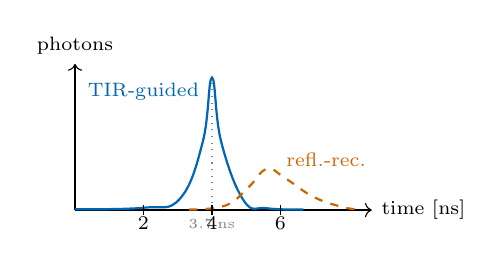
\begin{tikzpicture}[scale=0.58, every node/.style={font=\scriptsize}]
      % Schematic arrival spectrum (pure TikZ, no pgfplots)
      % Axes
      \draw[->] (0,0) -- (6.5,0) node[right] {time [ns]};
      \draw[->] (0,0) -- (0,3.2) node[above] {photons};
      % TIR peak at 3.0 (units: 1=1 ns here, peak at ~3.7ns -> scale 0.78)
      % Use plot coordinates to draw a Gaussian by hand (5 points)
      \draw[colEND,thick,smooth,tension=0.7]
        plot coordinates {(0,0.02)(1.5,0.05)(2.3,0.25)(2.8,1.5)(3.0,2.9)(3.2,1.5)(3.7,0.2)(4.2,0.04)(5.0,0.01)};
      \node[colEND] at (1.5,2.6) {TIR-guided};
      \draw[dotted,gray] (3.0,0) -- (3.0,3.0);
      \node[gray,font=\tiny] at (3.0,-0.3) {$3.7\ns$};
      % Reflector-recovered: broader, later, lower
      \draw[colTOP,thick,dashed,smooth,tension=0.7]
        plot coordinates {(2.5,0.01)(3.3,0.1)(3.8,0.5)(4.2,0.9)(4.6,0.7)(5.2,0.3)(5.8,0.08)(6.2,0.01)};
      \node[colTOP] at (5.5,1.1) {refl.-rec.};
      % Axis ticks
      \foreach \x/\l in {1.5/2,3.0/4,4.5/6}{
        \draw (\x,-0.1) -- (\x,0.1);
        \node at (\x,-0.3) {\l};
      }
    \end{tikzpicture}\\[2pt]
    \footnotesize Schematic. END timing is set by the TIR-guided peak.
  \end{columns}
\end{frame}

% ---- Bounces ----
\begin{frame}{Bounces and Reflector Attenuation}
  \begin{columns}[T]
    \column{0.50\linewidth}
    TIR photons zig-zag at angle $\alpha_c = 90^{\circ}-\theta_c = 50.73^{\circ}$ from the bar surface.\\[4pt]
    Number of bounces to traverse $L/2 = 700\mm$ on $H=10\mm$ faces:
    \[
      N_\text{bounce}^H = \frac{(L/2)\cdot\tan\alpha_c}{H} = \frac{700\times 1.223}{10} \approx \Nbounce
    \]
    For $W=60\mm$ faces: $N_\text{bounce}^W \approx \NbounceW$.\\[6pt]
    \textbf{Reflector attenuation length:}
    \[
      \Lambda_\text{refl} = \frac{H}{\tan\alpha_c\cdot\ln(1/R)} \approx \LambdaH
    \]
    {\footnotesize Napkin ($R=0.98$): $\Lambda_\text{refl}^H \approx \LambdaH$.
    Sim.\ data ($R=\Rvikuiti$): $\Lambda_\text{refl}^H \approx \NapLambdareflHmmsim$.}\\[2pt]
    At $L/2=700\mm$: survival $= 0.95^{85.6} \approx 1.2\%$.\\[4pt]
    \alert{Most photons reaching the END did \emph{not} bounce off the $H$-face Vikuiti.}

    \column{0.46\linewidth}
    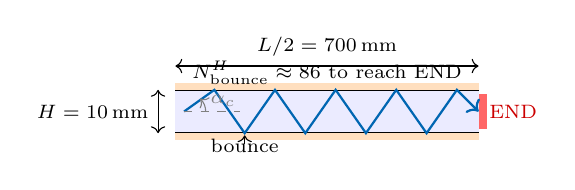
\begin{tikzpicture}[scale=0.55, every node/.style={font=\scriptsize}]
      % Zig-zag bounce diagram
      \fill[blue!8] (0,0) rectangle (7,1.0);
      \draw[thick] (0,0) -- (7,0);
      \draw[thick] (0,1.0) -- (7,1.0);
      \fill[orange!25] (0,1.0) rectangle (7,1.15);
      \fill[orange!25] (0,-0.15) rectangle (7,0);
      % SiPM at right end
      \fill[red!60] (7,0.1) rectangle (7.2,0.9);
      \node[red!80!black] at (7.8,0.5) {END};
      % zig-zag ray
      \draw[->,colEND,thick]
        (0.2,0.5) -- (0.9,1.0) -- (1.6,0) -- (2.3,1.0) -- (3.0,0) --
        (3.7,1.0) -- (4.4,0) -- (5.1,1.0) -- (5.8,0) -- (6.5,1.0) -- (7.0,0.5);
      % bounce labels
      \node at (1.6,-0.3) {bounce};
      \draw[->] (1.6,-0.25) -- (1.6,-0.05);
      % angle label
      \draw[dashed,gray] (0.2,0.5) -- (1.5,0.5);
      \draw[->,gray] (0.7,0.5) arc[start angle=0,end angle=48,radius=0.4];
      \node[gray] at (1.1,0.75) {$\alpha_c$};
      % N_bounce
      \node at (3.5,1.4) {$N_\text{bounce}^H \approx 86$ to reach END};
      \draw[<->] (0,1.55) -- (7,1.55) node[midway,above] {$L/2=700\mm$};
      % H dimension
      \draw[<->] (-0.4,0) -- (-0.4,1.0) node[midway,left] {$H=10\mm$};
    \end{tikzpicture}
    \vspace{2pt}
    \anafig{fig_survival_RN}
  \end{columns}
\end{frame}

% ---- Napkin photon budget ----
\begin{frame}{Napkin Photon Budget: Where Do the 19\,400 Photons Go?}
  \begin{columns}[T]
    \column{0.50\linewidth}
    MIP through $H=10\mm$ EJ-230: $\Delta E = 2.0\,\text{MeV}$.\\[4pt]
    {\small\begin{tabular}{lrl}
      \toprule
      Step & Photons & Factor\\
      \midrule
      Produced & 19\,400 & $Y \times \Delta E$ \\
      TIR toward 1 end & 5\,320 & $f_\text{TIR/end}$ \\
      Bulk survival & 2\,969 & $e^{-700/1200}$ \\
      At SiPM & 1\,425 & cov. $0.48$ \\
      Detected (PDE 0.40) & \textbf{570} & $\times 0.40$ \\
      \midrule
      \textbf{Geant4} & \textbf{701} & $+23\%$ \\
      \bottomrule
    \end{tabular}}\\[4pt]
    \alert{23\% surplus = reflector-recovered photons.}\\
    Napkin: TIR-only path.
    G4 includes Population II.

    \column{0.46\linewidth}
    \anafig{fig_bulk_survival}\\[-2pt]
    % Manual x-axis labels (ROOT only shows EJ-200)
    \begin{tikzpicture}[x=\linewidth, y=1cm, every node/.style={font=\tiny}]
      \node[blue!80!black]   at (0.22,0) {EJ-200};
      \node[green!60!black]  at (0.52,0) {EJ-204};
      \node[red!70!black]    at (0.82,0) {EJ-230};
    \end{tikzpicture}\\[-2pt]
    {\scriptsize\raggedright Bulk survival $e^{-L/(2\lambda)}$ at $x=0$ ($L/2=700\mm$).\par}
  \end{columns}
\end{frame}

% ---- Material comparison ----
\begin{frame}{Material Choice: EJ-230 is the Fastest Scintillator Here}
  \begin{columns}[T]
    \column{0.52\linewidth}
    \begin{tabular}{lccc}
      \toprule
      & EJ-200 & EJ-204 & \textbf{EJ-230} \\
      \midrule
      $\lambda_\text{att}$ [mm] & 3800 & 1600 & \textbf{1200} \\
      $\tau_\text{decay}$ [ns]  & 2.1  & 1.8  & \textbf{1.5} \\
      $\tau_\text{rise}$ [ns]   & 0.9  & 0.7  & \textbf{0.5} \\
      Yield [ph/MeV]            & 10000 & 10400 & 9700 \\
      $n$                       & 1.58  & 1.58  & 1.58 \\
      \midrule
      $N_\text{pe}$/end (G4)    & 1311  & 941  & \textbf{701} \\
      $\sigma_t$ ($x{=}0$) [ps]  & \RessigmabxzEROejA & \RessigmabxzEROejB & \textbf{\RessigmabxzEROejC}$^{\dagger}$ \\
      $\sigma_t$ (bar mean) [ps] & \RessigmabmEANejA  & \RessigmabmEANejB  & \textbf{\RessigmabmEANejC} \\
      \bottomrule
    \end{tabular}
    \vspace{4pt}\\
    \footnotesize $^\dagger$GEN-3 END-only (scan\_end\_vikuiti), $m^*$-opt.\\[4pt]
    $x=0$: EJ-230 (\RessigmaxzEROejC) $<$ EJ-204 (\RessigmaxzEROejB) $<$ EJ-200 (\RessigmaxzEROejA).\\
    Bar mean: EJ-230 (\RessigmamEANejC) $<$ EJ-200 (\RessigmamEANejA) $<$ EJ-204 (\RessigmamEANejB).

    \column{0.44\linewidth}
    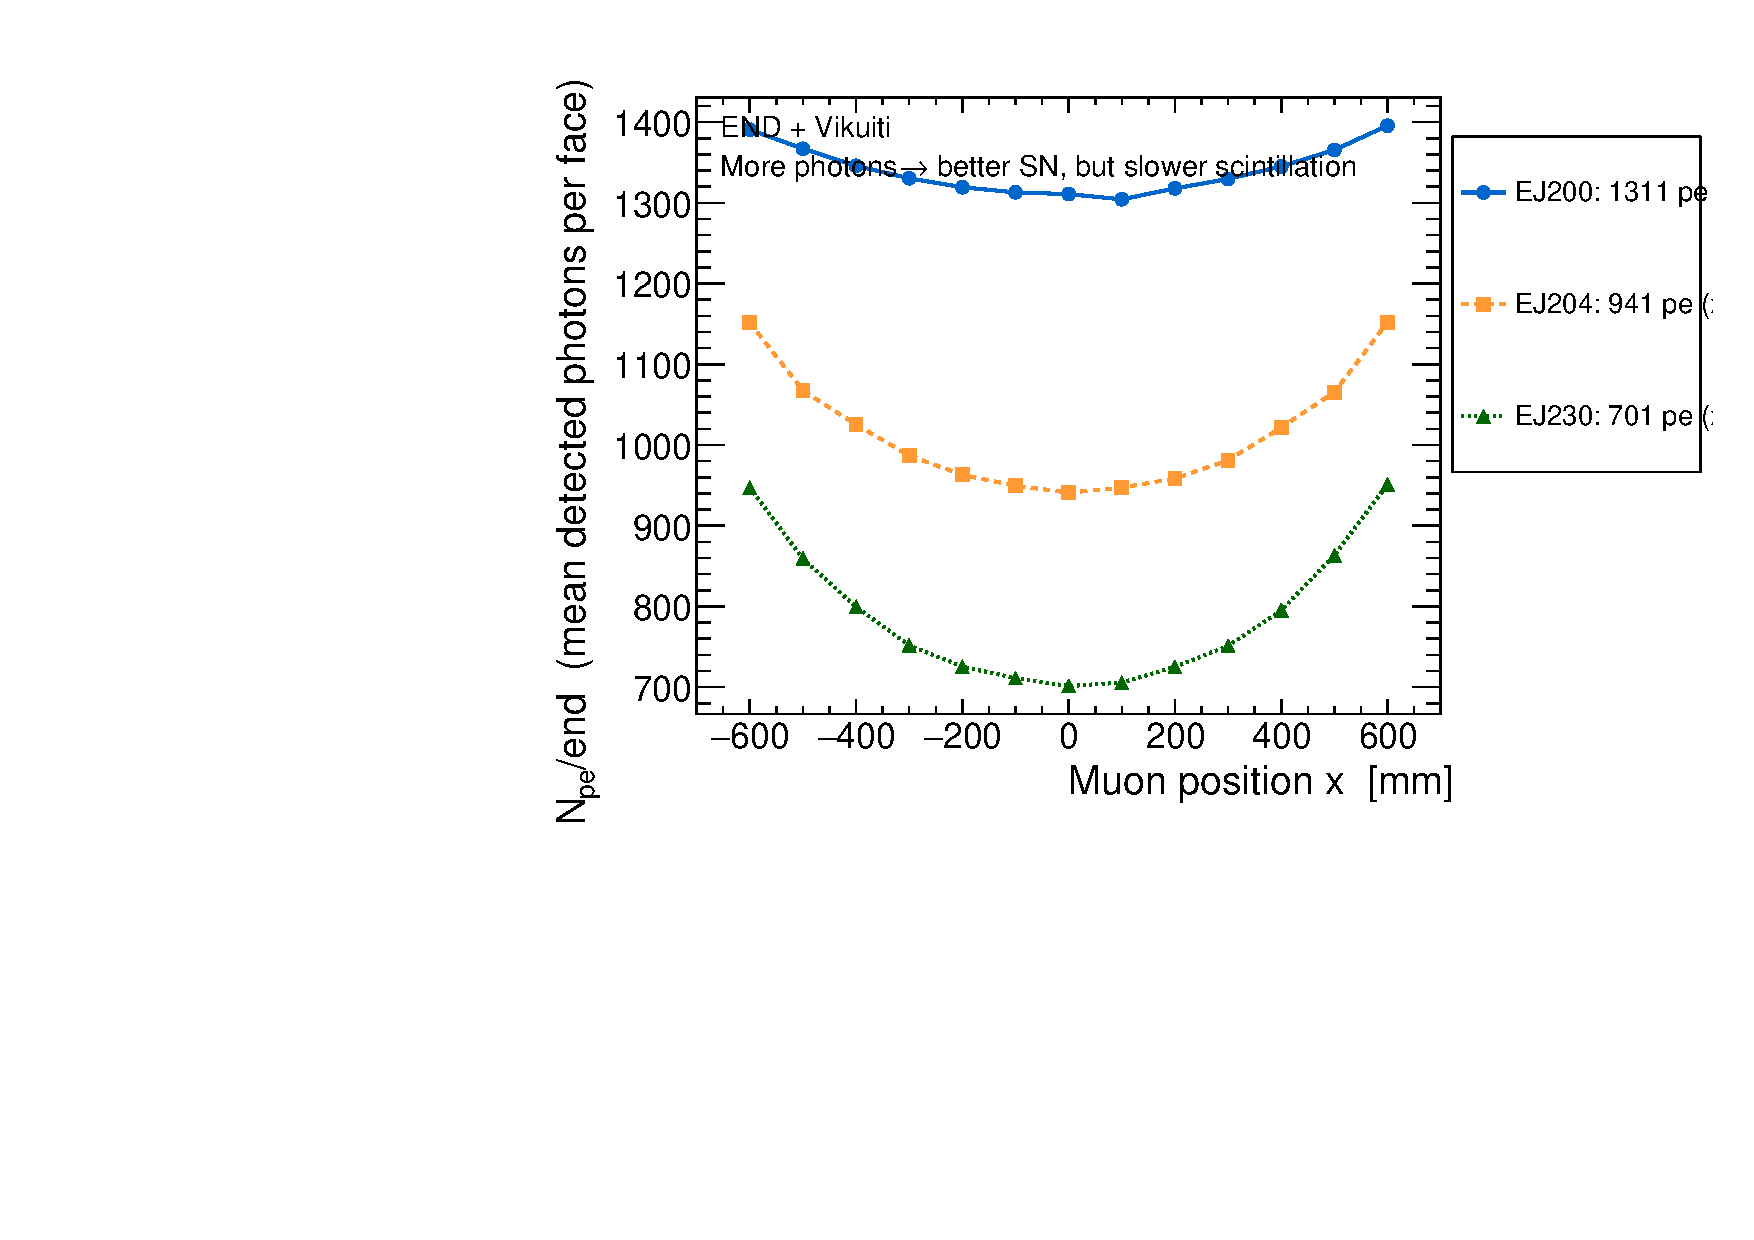
\includegraphics[width=0.82\linewidth]{figs/figM2_mat_npe}\\[1pt]
    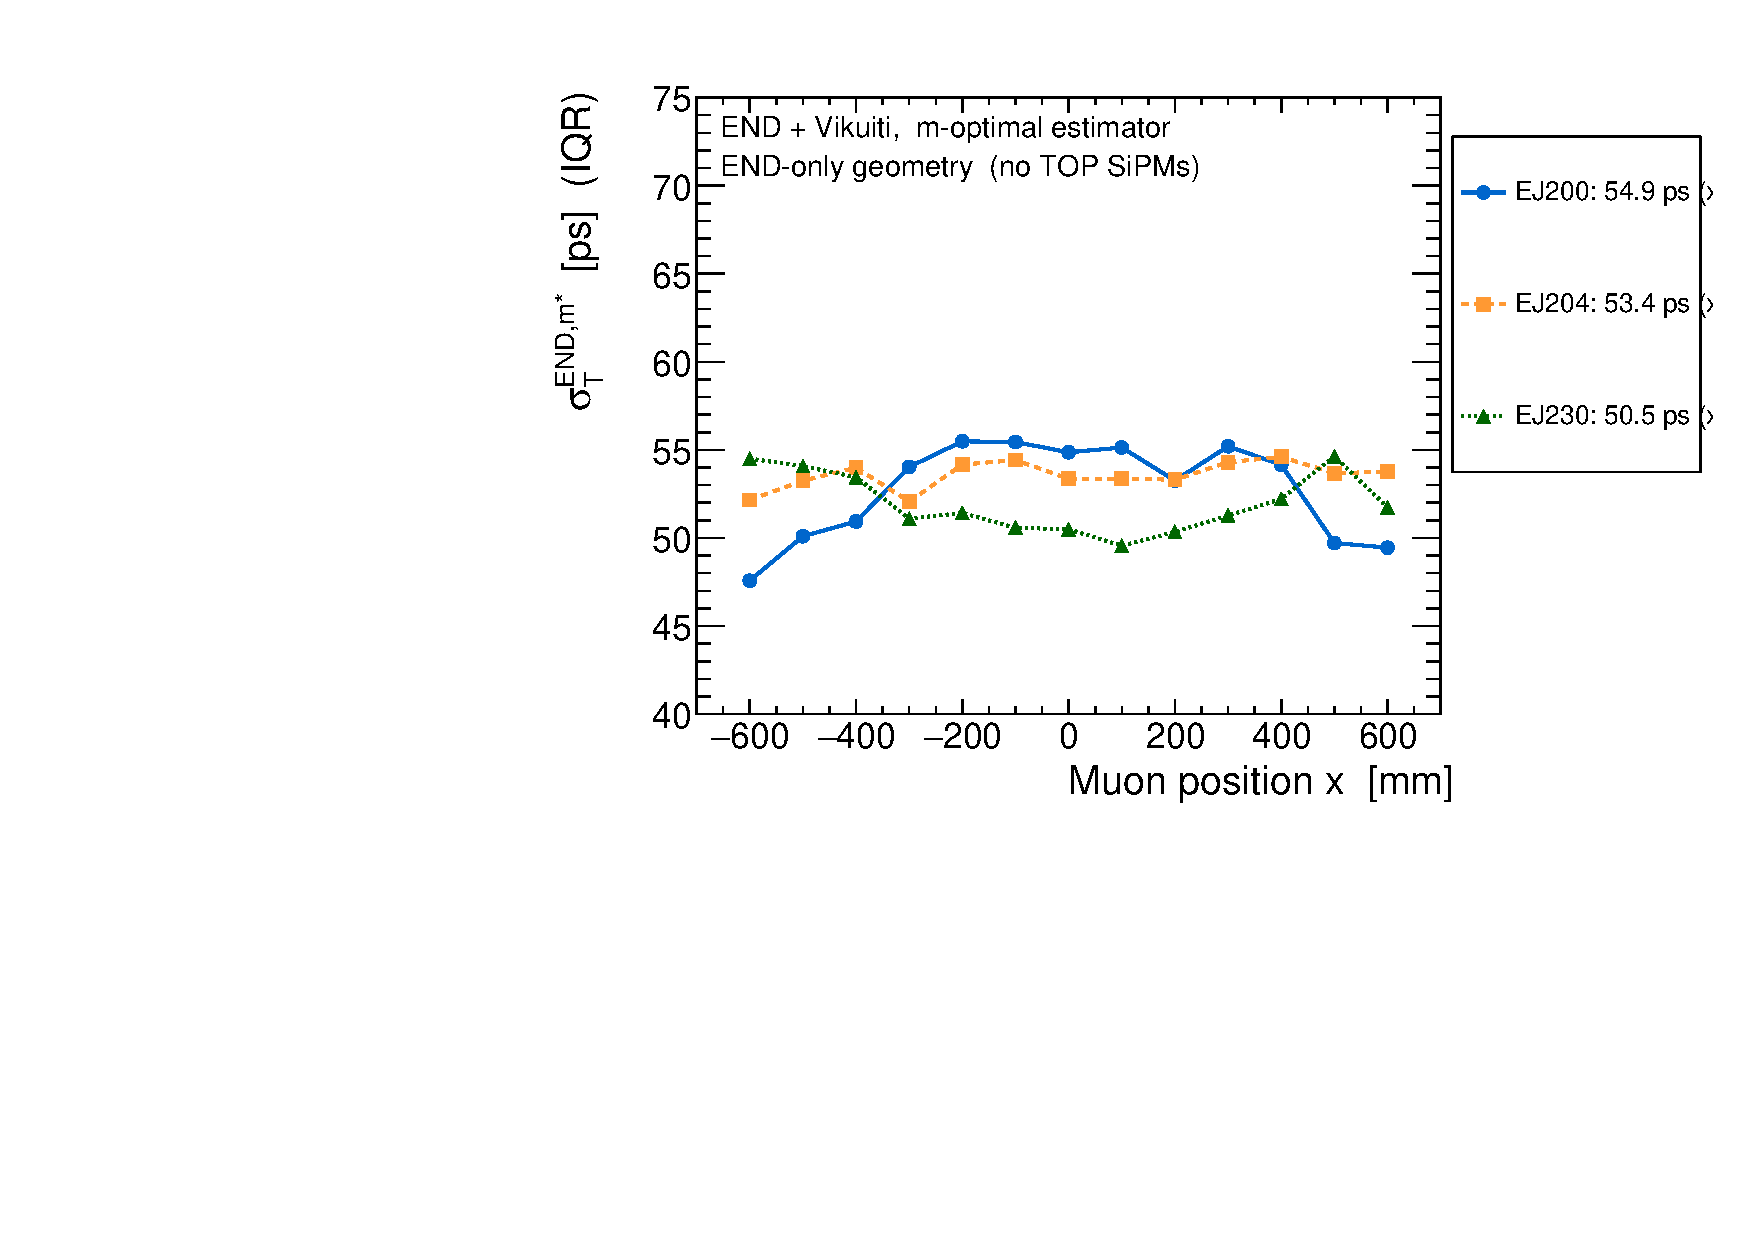
\includegraphics[width=0.82\linewidth]{figs/figM1_mat_sigma_end}
  \end{columns}
\end{frame}

% ====================================================================
\section{Geant4 Optical Model}
% ====================================================================

\begin{frame}{The Geant4 Optical Model (GEN-3)}
  \begin{columns}[T]
    \column{0.54\linewidth}
    \textbf{Current geometry (GEN-3):}
    \begin{itemize}\setlength\itemsep{2pt}
      \item Explicit \textbf{air gap} ($0.10\mm$) around bar
      \item Explicit \textbf{Mylar reflector} ($0.05\mm$) outside air
      \item Bar$\to$air: \texttt{CreateBarSurface()} — \texttt{dielectric\_dielectric, polished} → natural Fresnel + TIR for $\theta>\theta_c$
      \item Air$\to$Mylar: \texttt{CreateBarSkinReflector()} as border surface — \texttt{dielectric\_dielectric}, $R=0.95$ constant
      \item SiPM: \texttt{dielectric\_metal}, wavelength-dependent PDE (AFBR-S4N66P024M)
    \end{itemize}
    \vspace{4pt}
    \alert{Key:} the bar–air surface implements \emph{natural} Fresnel TIR.
    No artificial reflectivity is set on the bar itself.
    Vikuiti only acts on photons that escape the bar.

    \column{0.42\linewidth}
    % Air-gap vs skin-surface comparison
    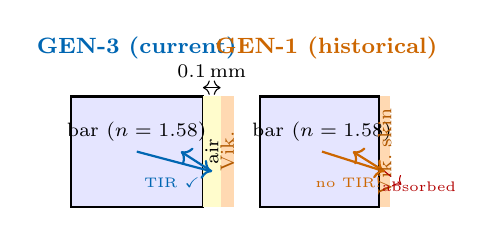
\begin{tikzpicture}[scale=0.56, every node/.style={font=\scriptsize}]
      % --- Left: GEN-3 geometry (air gap) ---
      \node[font=\footnotesize\bfseries, colEND] at (1.5,3.6) {GEN-3 (current)};
      \fill[blue!10] (0,0) rectangle (3,2.5);
      \draw[thick] (0,0) rectangle (3,2.5);
      \fill[yellow!20] (3,0) rectangle (3.4,2.5);
      \fill[orange!30] (3.4,0) rectangle (3.7,2.5);
      \draw[colEND,thick,->] (1.5,1.25) -- (3.2,0.8);
      \draw[colEND,thick,->] (3.2,0.8) -- (2.5,1.25);
      \node at (1.5,1.7) {bar ($n=1.58$)};
      \node[rotate=90] at (3.2,1.25) {air};
      \node[orange!70!black,rotate=90] at (3.55,1.25) {Vik.};
      \draw[<->] (3,2.7) -- (3.4,2.7) node[midway,above] {$0.1\mm$};
      \node[colEND,font=\tiny] at (2.3,0.55) {TIR $\checkmark$};
      % --- Right: historical skin surface ---
      \node[font=\footnotesize\bfseries, colTOP] at (5.8,3.6) {GEN-1 (historical)};
      \fill[blue!10] (4.3,0) rectangle (7,2.5);
      \fill[orange!30] (7,0) rectangle (7.25,2.5);
      \draw[thick] (4.3,0) rectangle (7,2.5);
      \draw[colTOP,thick,->] (5.7,1.25) -- (7.12,0.8);
      \draw[colTOP,thick,->] (7.12,0.8) -- (6.4,1.25);
      \node at (5.7,1.7) {bar ($n=1.58$)};
      \node[orange!70!black,rotate=90] at (7.12,1.25) {Vik.\ skin};
      \node[colTOP,font=\tiny] at (6.3,0.55) {no TIR!};
      \draw[->,red!70!black,dashed] (7.12,0.8) -- (7.5,0.5);
      \node[red!70!black,font=\tiny] at (7.9,0.45) {absorbed};
    \end{tikzpicture}
    \vspace{2pt}\\
    \footnotesize GEN-1 skin surface on bar eliminates TIR entirely → photon deficit ($\times 1500$, see B2).
  \end{columns}
\end{frame}

\begin{frame}{Geant4 Validates the Napkin}
  \begin{columns}[T]
    \column{0.50\linewidth}
    \textbf{Photon yield at $x=0$, EJ-230:}\\[4pt]
    \begin{tabular}{lcc}
      \toprule
      Path & Napkin & G4 \\
      \midrule
      TIR-guided / end & 570 & — \\
      Reflector-recovered & 0 & — \\
      \textbf{Total / end} & \textbf{570} & \textbf{701.3} \\
      \bottomrule
    \end{tabular}\\[1pt]
    $\Delta N_\text{pe}/N_\text{nap} = +23\%$.\\[4pt]
    Napkin accuracy: $-17\%$ (predicted deficit).
    \emph{Reason:} napkin counts only the TIR-guided population.
    Reflector-recovered photons add a systematic $+23\%$ that the napkin cannot predict without knowing $R$.\\[6pt]
    \textbf{Timing estimate (napkin, order-of-magnitude):}
    \[
      \sigma_t \approx \frac{\tau_\text{decay}}{\sqrt{N_\text{pe}}}
      = \frac{1500\,\text{ps}}{\sqrt{570}} \approx 63\,\text{ps}
    \]
    Geant4 (hybrid geometry, $N_\text{TOP}=20$, $m=8$): $\sigma_\text{END} = \sigmaENDval$ — within 20\%.
    {\footnotesize END-only ($N_\text{TOP}=0$, $m^*=7$): $\sigmaENDonlyval$ (scan\_end\_vikuiti).}

    \column{0.46\linewidth}
    \anafig{fig_npe_x}\\[1pt]
    \footnotesize $N_\text{pe}$/end vs $x$ for three scintillators.
    EJ-200 highest, EJ-230 lowest but fastest decay.
  \end{columns}
\end{frame}

% ====================================================================
\section{Estimators}
% ====================================================================

\begin{frame}{END Estimator: m-Average of First Photons}
  \begin{columns}[T]
    \column{0.52\linewidth}
    \textbf{Definition:}
    \[
      T_0^\text{END} = \tfrac{1}{2}\!\left(\bar{t}_L^{(m)} + \bar{t}_R^{(m)}\right),
      \quad
      \bar{t}^{(m)} = \frac{1}{m}\sum_{i=1}^{m} t_i^{(\text{sorted})}
    \]
    Average of first $m$ photon arrival times per END face.\\[4pt]
    \textbf{Optimal $m$:} balance between noise rejection (large $m$) and avoiding slow photons (small $m$). Oracle: $m^* = 8$ at $x=0$.\\[4pt]
    \textbf{Result at $x=0$, $m=8$:}
    \[
      \sigma_\text{END} = \sigmaENDval
    \]
    \textbf{Path to END:} $L/2 = \NapLhalfmm$ axial (\NaptaxialENDns) up to $(L/2)/\!\sin\theta_c = \NappathTIRlimmm$ at $\theta_c$ from the $H$-face normal (\NaptTIRlimns).

    \column{0.44\linewidth}
    \anafig{fig_end_mscan}\\[2pt]
    \footnotesize $\sigma_\text{END}$ vs $m$ at $x=0$. Minimum near $m=8$.
  \end{columns}
\end{frame}

\begin{frame}{TOP Estimator: $k$-th Order Statistic of Pooled Hits}
  \begin{columns}[T]
    \column{0.52\linewidth}
    \textbf{Definition:}
    \[
      T_0^\text{TOP} = t_{(k)}^\text{pool}
    \]
    $k$-th smallest arrival time among \emph{all} TOP SiPMs pooled together.\\[4pt]
    \textbf{Key difference from END:}
    TOP SiPMs sit along the bar; a hit on the nearest SiPM travels only $\sim\!10\mm$ (path $\approx 13\mm$).
    \[
      \tau_\text{prop}^\text{TOP} \approx \frac{10\mm}{v_g} = 53\ps
    \]
    vs.\ $\tau_\text{prop}^\text{END} \in [\NaptaxialENDns,\,\NaptTIRlimns]$.\\[4pt]
    \textbf{Result at $x=0$, $k=3$, $N_\text{TOP}=20$:}
    \[
      \sigma_\text{TOP} = \sigmaTOPval
    \]
    \alert{3.5× better than END.} The key is proximity, not photon statistics.

    \column{0.44\linewidth}
    \anafig{fig1_kscan}\\[2pt]
    \footnotesize $\sigma_\text{TOP}$ vs $k$ at $x=0$, $N_\text{TOP}=20$. Minimum at $k=3$.
  \end{columns}
\end{frame}

\begin{frame}{Why TOP Beats END: Near-Field vs Far-Field}
  \begin{columns}[T]
    \column{0.56\linewidth}
    \textbf{Propagation jitter} — not photon counting — limits END timing.\\[4pt]
    \begin{tabular}{lcc}
      \toprule
      & END & TOP \\
      \midrule
      Path length & $\NapLhalfmm$--$\NappathTIRlimmm$ & $\sim\!13\mm$ \\
      $\tau_\text{prop}$ & $\NaptaxialENDns$--$\NaptTIRlimns$ & $\sim\!53\ps$ \\
      Path dispersion & large & negligible \\
      $N_\text{pe}$ used & $\sim\!8$ & $\sim\!3$ (pooled) \\
      $\sigma_t$ at $x=0$ & $53.7\ps$ & $15.2\ps$ \\
      \bottomrule
    \end{tabular}\\[3pt]
    {\footnotesize $m=8$ average uses earliest photons, near the axial bound (\NaptaxialENDns).}\\[3pt]
    The TOP SiPM nearest to the muon hit position receives photons that have traveled almost no distance.
    The 3rd-order statistic (out of $\sim\!100$ pooled photons) suppresses random single-photon fluctuations.\\[6pt]
    \alert{The factor 3.5× improvement is purely from geometry, not hardware.}

    \column{0.40\linewidth}
    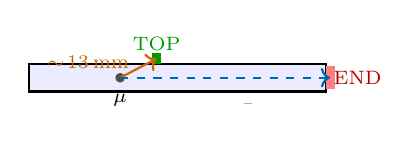
\begin{tikzpicture}[scale=0.58, every node/.style={font=\scriptsize}]
      % Near-field vs far-field schematic
      \fill[blue!8] (0,0) rectangle (6.5,0.6);
      \draw[thick] (0,0) rectangle (6.5,0.6);
      % END SiPM
      \fill[red!50] (6.5,0.05) rectangle (6.7,0.55);
      \node[red!70!black] at (7.2,0.3) {END};
      % TOP SiPM
      \fill[green!60!black] (2.7,0.6) rectangle (2.9,0.85);
      \node[green!60!black] at (2.8,1.05) {TOP};
      % Muon hit
      \fill[black!70] (2.0,0.3) circle(3pt);
      \node at (2.0,-0.2) {$\mu$};
      % Near-field arrow
      \draw[->,colTOP,thick] (2.0,0.3) -- (2.8,0.72);
      \node[colTOP] at (1.3,0.65) {$\sim\!13\mm$};
      % Far-field arrow
      \draw[->,colEND,thick,dashed] (2.0,0.3) -- (6.6,0.3);
      \node[colEND,font=\tiny] at (4.8,-0.28) {$\NapLhalfmm$--$\NappathTIRlimmm$};
    \end{tikzpicture}\\[4pt]
    \footnotesize The nearest TOP SiPM is at most $35\mm$ from any muon hit ($N=20$).
  \end{columns}
\end{frame}

% ====================================================================
\section{Effective Velocity \& BLUE}
% ====================================================================

\begin{frame}{Effective Velocity: $v_\text{eff} = \veffEND$}
  \begin{columns}[T]
    \column{0.48\linewidth}
    From END $\Delta t = t_R^{(m)} - t_L^{(m)}$ vs hit position $x$:
    \[
      \langle \Delta t(x)\rangle = a + \frac{x}{v_\text{eff}/2}
    \]
    \textbf{Fit} ($m=8$, EJ-230, $N_\text{TOP}=20$):
    \begin{itemize}\setlength\itemsep{1pt}
      \item $v_\text{eff} = \veffEND$
      \item $a = 0.44\pm 0.38\ps$
      \item $\chi^2/\text{ndf} = 1250/11$, $p\approx 0$
      \item Residual RMS $= 14.5\ps$
    \end{itemize}
    \alert{Highly significant nonlinearity.} S-shape pattern driven by photon pool edge asymmetry.\\[4pt]
    \textbf{Compare:} $v_g = \vgroup$; $v_\text{eff} < v_g$ because $m=8$ average includes photons that bounced more.\\[4pt]
    Position resolution: $\sigma_x = \frac{v_\text{eff}}{2}\sigma_{\Delta t} = \sigmax$.

    \column{0.48\linewidth}
    
\includegraphics[width=0.92\linewidth]{figs/v5_veff_fit}\\[1pt]
    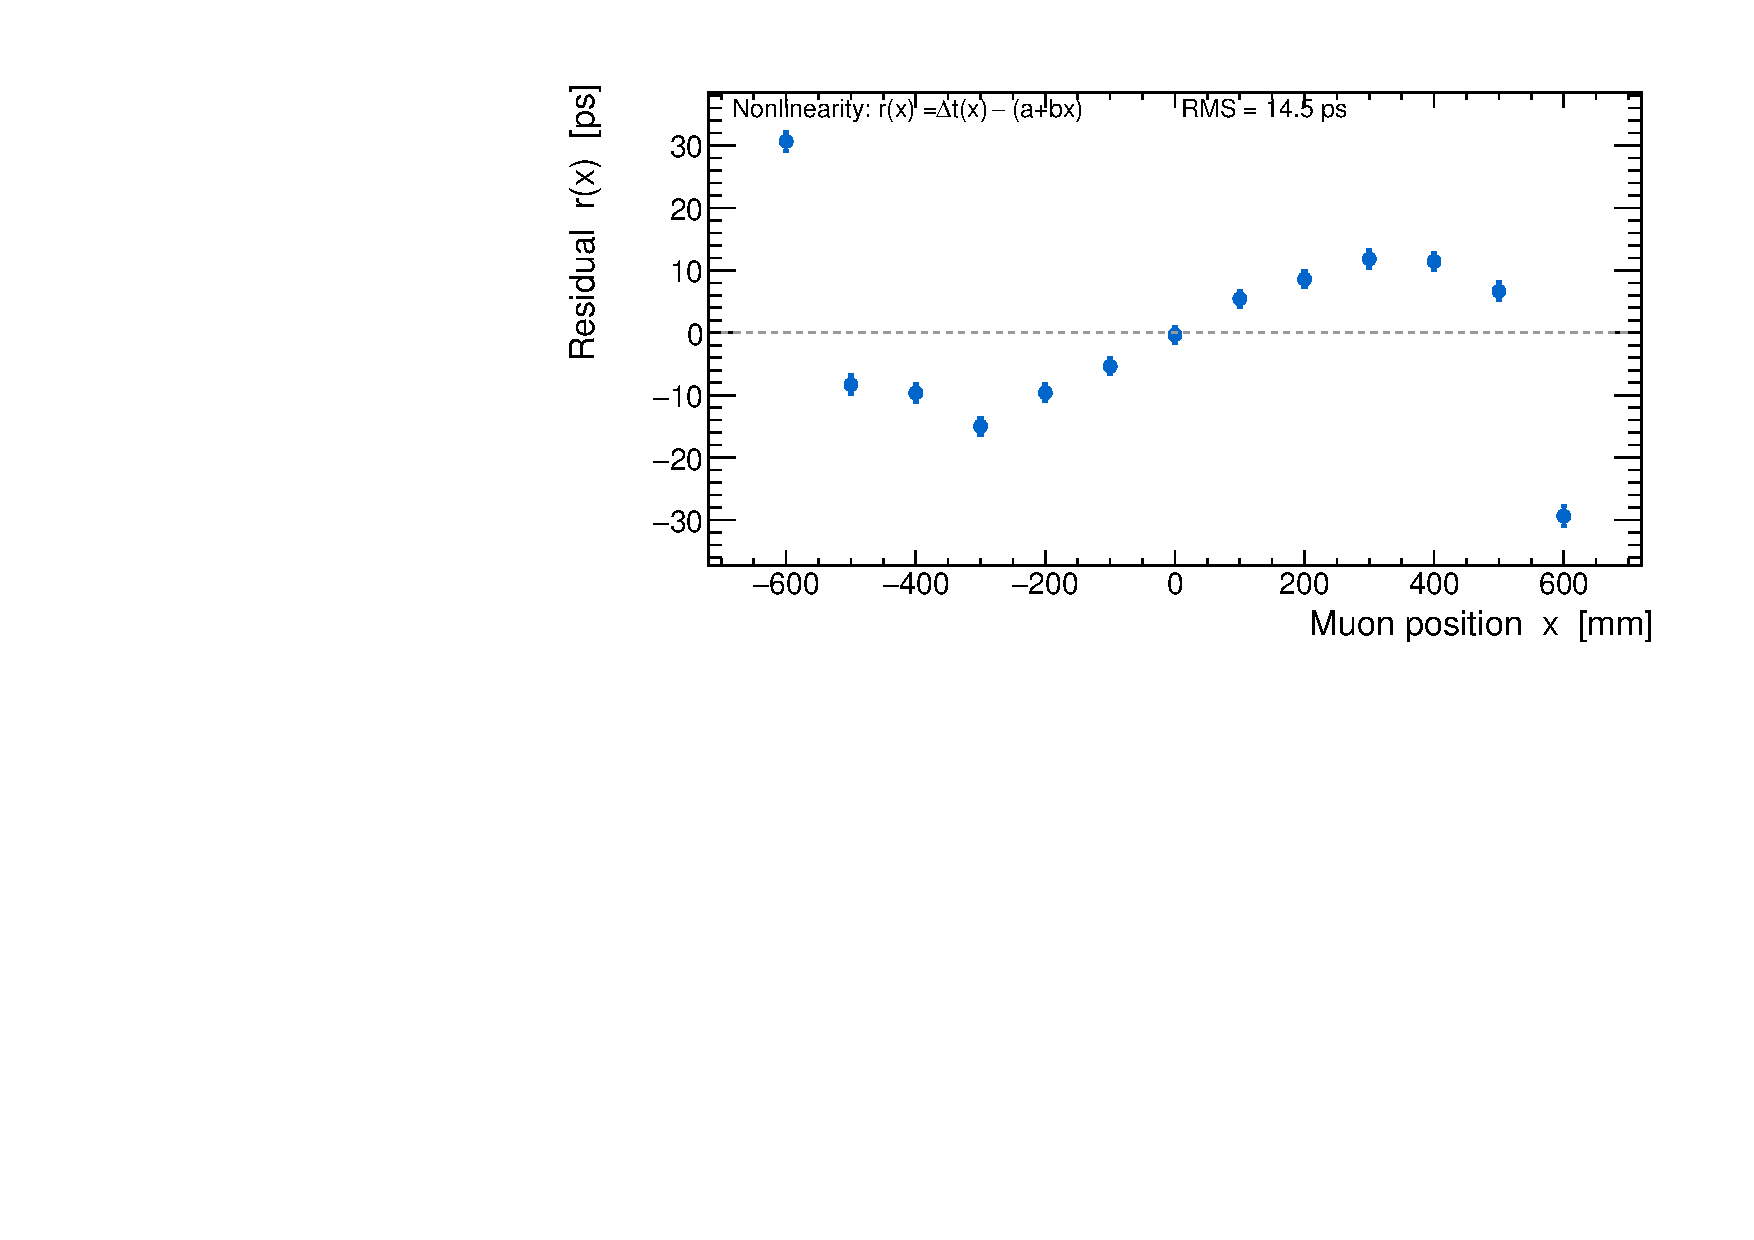
\includegraphics[width=0.92\linewidth]{figs/v5_veff_residual}
  \end{columns}
\end{frame}

\begin{frame}[shrink=3]{BLUE Combination: TOP Estimator Dominates}
  \begin{columns}[T]
    \column{0.56\linewidth}
    \textbf{BLUE (Best Linear Unbiased Estimator):}
    \[
      T_0^\text{BLUE} = w_\text{END}\,T_0^\text{END} + w_\text{TOP}\,T_0^\text{TOP}
    \]
    Weights from covariance matrix ($\sigma^2 = \sigma_\text{IQR}^2$, $C_{ET}=\text{Cov}(T_E,T_T)$ empirical):
    \[
      w_\text{END} = \frac{\sigma_T^2 - C_{ET}}{\sigma_E^2 + \sigma_T^2 - 2\,C_{ET}}
    \]
    At $x=0$, $k=3$, $m=8$, $N_\text{TOP}=20$:
    \begin{center}
    \begin{tabular}{lc}
      \toprule
      Quantity & Value \\
      \midrule
      $\sigma_\text{END}$ & $\sigmaENDval$ \\
      $\sigma_\text{TOP}$ & $\sigmaTOPval$ \\
      $C_{ET}$ & $196.3\,\text{ps}^2$ \\
      $w_\text{END}$ & ${\lesssim}\,0.1$ (not resolved, $n=5000$) \\
      $\sigma_\text{BLUE}$ & $\mathbf{\sigmaBLUEval}$ \\
      \bottomrule
    \end{tabular}
    \end{center}
    {\footnotesize $\sigma_\text{BLUE}^\text{formula}$ ($w_\text{END}=0.013$, mixed cov.) $= 15.18\ps$;
    $\sigma_\text{IQR}^\text{event} = 15.21\ps$.
    Different scale metrics of a heavy-tailed distribution — not a consistency check.}

    \column{0.40\linewidth}
    \textbf{Why does TOP dominate?}\\[2pt]
    $\sigma_\text{TOP}^2 \ll \sigma_\text{END}^2$: the END estimator is so much worse that it contributes almost nothing to the BLUE combination.\\[5pt]
    \alert{The BLUE estimator is, to excellent approximation, just the TOP estimator.}\\[5pt]
    $\sigma_\text{BLUE}$ and $\sigma_\text{TOP}$ differ by less than one bootstrap standard error (${\approx}0.17\ps$ at $n=5000$).\\[5pt]
    $w_\text{END}$ \textbf{not resolved} at $n=5000$: IQR flat to within errors over $w\in[0,0.1]$ (total variation $0.26\ps$). See App.~G2.
  \end{columns}
\end{frame}

% ====================================================================
\section{Performance vs Position}
% ====================================================================

\begin{frame}{Global Performance (Deployable: $k=3$, $m=8$)}
  \begin{columns}[T]
    \column{0.52\linewidth}
    \textbf{Fixed parameters} across all positions — deployable in real detector.\\[4pt]
    \begin{tabular}{ccccc}
      \toprule
      $x$ [mm] & $\sigma_E$ & $\sigma_T$ & $\sigma_B$ & $w_E$ \\
      \midrule
      $-600$ & 59.3 & 16.3 & 16.7 & 0.115 \\
      $-500$ & 61.0 & 23.2 & 24.6 & 0.208 \\
      $-400$ & 56.7 & 17.0 & 18.1 & 0.178 \\
      $-300$ & 56.7 & 17.3 & 18.6 & 0.183 \\
      $-200$ & 53.6 & 23.2 & 24.5 & 0.237 \\
      $0$    & 53.7 & 15.2 & \textbf{15.0} & 0.086 \\
      $+600$ & 61.0 & 16.8 & 16.9 & 0.118 \\
      \bottomrule
    \end{tabular}
    \footnotesize All $\sigma$ in ps. $N_\text{TOP}=20$, EJ-230.
    $\dagger$$w_E$ computed position-by-position with np.var(); best-estimate IQR-based $w_E{\lesssim}\,0.1$ at $x=0$ (not resolved at $n=5000$, see App.~G2).\\[6pt]
    \alert{Peaks at $x=\pm200,\pm500\mm$}: $k=3$ is locally suboptimal there.
    Mean $\sigma_\text{BLUE}=19.5\ps$ across bar.\\[3pt]
    {\footnotesize $\sigma_B(x{=}0)=15.0\ps$ (v5, \texttt{np.var} weights) vs $15.21\ps$ (best-estimate IQR weights); definitional, see App.~G2.}

    \column{0.44\linewidth}
    \anafig{v5_sigma_vs_x}\\
    \footnotesize Blue = global ($k=3$, $m=8$); gray = oracle ($k^*(x)$, $m^*(x)$).
  \end{columns}
\end{frame}

\begin{frame}{Oracle vs Global: The Deployment Cost}
  \begin{columns}[T]
    \column{0.50\linewidth}
    \textbf{Oracle}: locally optimal $(k^*(x),m^*(x))$ — requires knowing muon position.
    Not deployable, but a diagnostic lower bound.\\[4pt]
    \begin{tabular}{ccc}
      \toprule
      & Global & Oracle \\
      \midrule
      $\sigma_\text{BLUE}$ at $x=0$ & 15.0 & 15.0 \\
      Mean $\sigma_\text{BLUE}$ & 19.5 & 16.1 \\
      Min $\sigma_\text{BLUE}$ & 15.0 & 14.7 \\
      Max $\sigma_\text{BLUE}$ & 24.7 & 18.5 \\
      \midrule
      \textbf{Gap (mean)} & \multicolumn{2}{c}{\textbf{3.4 ps}} \\
      \bottomrule
    \end{tabular}
    \footnotesize All ps. $N_\text{TOP}=20$, EJ-230.\\[6pt]
    The 3.4 ps gap is the cost of deploying fixed $k=3,m=8$ parameters across all positions.\\[4pt]
    \alert{At $x=0$: global = oracle ($k^*=3$, $m^*=8$).}\\
    Peaks at $x=\pm200,\pm500\mm$ arise because $k^*=2$ is better there but global uses $k=3$.\\[3pt]
    {\footnotesize $\sigma_B(x{=}0)=15.0\ps$ (v5, \texttt{np.var} weights) vs $15.21\ps$ (best-estimate IQR weights); definitional, see App.~G2.}

    \column{0.46\linewidth}
    \textbf{Oracle $k^*(x)$:}
    \begin{center}
    \begin{tabular}{cc}
      \toprule
      $x$ [mm] & $(k^*, m^*)$ \\
      \midrule
      $-600$ & $(2,10)$ \\
      $-500$ & $(1,11)$ \\
      $0$    & $(3,8)$  \\
      $+500$ & $(1,5)$  \\
      $+600$ & $(2,5)$  \\
      \bottomrule
    \end{tabular}
    \end{center}
    \vspace{4pt}
    $k^*=1$ (first photon) at bar edges where TOP photons arrive sparsely.
    $k^*=3$ at bar center where $N_\text{TOP}$ pool is densest.
  \end{columns}
\end{frame}

% ====================================================================
\section{Channel Optimisation}
% ====================================================================

\begin{frame}{$N_\text{TOP}$ Scan: Physical Geometry Simulations}
  \begin{columns}[T]
    \column{0.52\linewidth}
    Each $N_\text{TOP}$ value uses its own simulated file with SiPMs physically placed at correct positions. Not software ablation.\\[6pt]
    \begin{tabular}{ccccc}
      \toprule
      $N_\text{TOP}$ & $N_\text{ch}$ & $k^*$ & $\sigma_\text{TOP}$ & $\sigma_\text{BLUE}$ \\
      \midrule
      4  & 20 & 1 & 78.2 & 45.3 \\
      8  & 24 & 1 & 32.0 & 32.2 \\
      14 & 30 & 2 & 18.7 & 18.4 \\
      \textbf{20} & \textbf{36} & \textbf{3} & \textbf{15.2} & \textbf{15.0} \\
      \bottomrule
    \end{tabular}
    \footnotesize All $\sigma$ in ps. $m=8$, EJ-230, $x=0$. $N_\text{ch} = 16+N_\text{TOP}$.\\[6pt]
    END-only ($N_\text{TOP}=0$): $\sigma \approx 50.5\ps$.\\[4pt]
    Adding TOP SiPMs: $50.5 \to 45.3 \to 32.2 \to 18.4 \to 15.0\ps$.

    \column{0.44\linewidth}
    \anafig{v5_pareto}\\[2pt]
    \footnotesize $\sigma_\text{BLUE}$ vs $N_\text{ch}$. Elbow at $N_\text{TOP}=14$ ($N_\text{ch}=30$).
    20 TOP channels for last 3.4 ps gain.
  \end{columns}
\end{frame}

% ====================================================================
\section{Position Measurement}
% ====================================================================

\begin{frame}{Position Measurement: END $\Delta t$ is the Right Method}
  \begin{columns}[T]
    \column{0.50\linewidth}
    \textbf{END $\Delta t$ method:}
    \[
      x_\text{rec} = \frac{v_\text{eff}}{2}\cdot\Delta t,\quad
      \sigma_x = \frac{v_\text{eff}}{2}\,\sigma_{\Delta t}
    \]
    At $m=8$: $\sigma_x = \sigmax$ with $v_\text{eff}=\veffEND$.\\
    No edge bias. Linear calibration.\\[8pt]
    \textbf{TOP $N_\text{pe}$ centroid (LOO):}
    \[
      x_\text{centroid} = \frac{\sum_i x_i N_i}{\sum_i N_i}
    \]
    Leave-one-out cross-validation on 12/13 positions.
    Result: $\sigma_x = 17.2\mm$ (linear fit), \alert{$+29\mm$ bias at bar ends.}\\[4pt]
    \alert{END method is 2× better with no edge bias.}

    \column{0.46\linewidth}
    \anafig{v5_top_position_loo}\\[2pt]
    \footnotesize TOP centroid LOO: large edge bias at $x=\pm600\mm$.
    $x_\text{true}=\pm600\mm \to x_\text{centroid}\approx\pm313\mm$ (saturation).
  \end{columns}
\end{frame}

% ====================================================================
\section{Design Summary}
% ====================================================================

\begin{frame}{Design Decision: EJ-230 + 20 TOP + 16 END}
  \begin{columns}[T]
    \column{0.52\linewidth}
    \textbf{Selected configuration:}
    \begin{itemize}\setlength\itemsep{3pt}
      \item Scintillator: \textbf{EJ-230} ($\tau=1.5\ns$, $\lambda_\text{att}=1200\mm$)
      \item Reflector: \textbf{Vikuiti ESR} ($R=\Rvikuiti$ in data; code $0.98$ since \texttt{c7acb7a})
      \item END SiPMs: \textbf{8 per face} = 16 total
      \item TOP SiPMs: \textbf{20 along bar} (step $\approx\!70\mm$)
      \item Total channels: \textbf{36}
    \end{itemize}
    \vspace{4pt}
    \textbf{Performance (global $k=3$, $m=8$):}
    \begin{center}
    \begin{tabular}{lc}
      \toprule
      Quantity & Value \\
      \midrule
      $\sigma_t$ at $x=0$ & $\mathbf{15.2\ps}$ \\
      Mean $\sigma_t$ across bar & $19.5\ps$ \\
      $\sigma_x$ (END $\Delta t$) & $\mathbf{7.9\mm}$ \\
      $N_\text{pe}$/end at $x=0$ & $701.3$ \\
      \bottomrule
    \end{tabular}
    \end{center}
    Target: $\sigma_t < 100\ps$. \alert{Achieved: $15.2\ps$ — 6.6× better than target.}

    \column{0.44\linewidth}
    \textbf{Path to this result:}\\[3pt]
    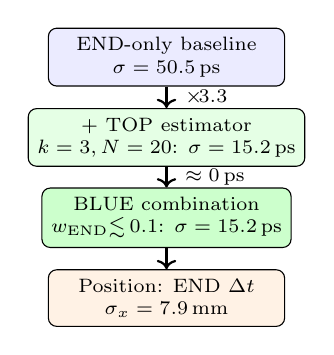
\begin{tikzpicture}[scale=0.60, every node/.style={font=\scriptsize},
      box/.style={draw,rounded corners=3pt,fill=blue!8,minimum width=3.0cm,minimum height=0.55cm,align=center}]
      \node[box] (a) at (0,7.2) {END-only baseline\\$\sigma=50.5\ps$};
      \node[box,fill=green!10] (b) at (0,5.5) {+ TOP estimator\\$k=3,N=20$: $\sigma=15.2\ps$};
      \node[box,fill=green!20] (c) at (0,3.8) {BLUE combination\\$w_\text{END}{\lesssim}\,0.1$: $\sigma=15.2\ps$};
      \node[box,fill=orange!10] (d) at (0,2.1) {Position: END $\Delta t$\\$\sigma_x=7.9\mm$};
      \draw[->,thick] (a)--(b) node[midway,right,xshift=3pt] {$\times\!3.3$};
      \draw[->,thick] (b)--(c) node[midway,right,xshift=3pt] {$\approx 0\ps$};
      \draw[->,thick] (c)--(d);
    \end{tikzpicture}\\[3pt]
    {\small $\times\!3.3$ = TOP geometry (near-field path).\\
    BLUE: essentially free combination.}
  \end{columns}
\end{frame}

\begin{frame}{Summary}
  \begin{block}{Napkin first — Geant4 second}
    First-principles predictions (TIR, bounce counting, photon budget) correctly set the order of magnitude
    and explain the trends. Geant4 confirms quantitatively and reveals the reflector-recovered contribution.
  \end{block}
  \vspace{4pt}
  \begin{columns}[T]
    \column{0.48\linewidth}
    \textbf{Optical physics:}
    \begin{itemize}\setlength\itemsep{2pt}
      \item TIR traps 54.8\% of photons toward ends
      \item Vikuiti (R=0.95) recovers non-TIR photons (+23\%)
      \item EJ-230 is fastest despite lower yield
    \end{itemize}
    \textbf{Estimators:}
    \begin{itemize}\setlength\itemsep{2pt}
      \item END m-avg ($m=8$): $\sigma=53.7\ps$
      \item TOP $k$-th order ($k=3$, $N=20$): $\sigma=15.2\ps$
      \item BLUE: $\sigma=15.2\ps$, $w_\text{END}{\lesssim}\,0.1$ (END contributes marginally)
    \end{itemize}

    \column{0.48\linewidth}
    \textbf{Optimisation:}
    \begin{itemize}\setlength\itemsep{2pt}
      \item Global ($k=3,m=8$): mean $19.5\ps$, deployable
      \item Oracle lower bound: mean $16.1\ps$ ($-3.4\ps$ gap)
      \item Pareto elbow at $N_\text{TOP}=14$; $N=20$ for best performance
    \end{itemize}
    \textbf{Position:}
    \begin{itemize}\setlength\itemsep{2pt}
      \item END $\Delta t$: $\sigma_x=7.9\mm$, no edge bias
      \item TOP centroid: $\sigma_x=17.2\mm$, $+29\mm$ edge bias
    \end{itemize}
    \vspace{4pt}
    \alert{Design: EJ-230, 36 channels (16 END + 20 TOP), $\sigma_t=15.2\ps$.}
  \end{columns}
\end{frame}

% ====================================================================
% APPENDIX
% ====================================================================
\appendix

\begin{frame}{}
  \begin{center}
    \Large\bfseries Appendix\\[8pt]
    \normalsize Technical backup slides
  \end{center}
\end{frame}

% ---- Appendix A: Optical model ----
\begin{frame}{A1 — Geant4 Surface Definitions}
  \begin{columns}[T]
    \column{0.55\linewidth}
    \textbf{CreateBarSurface()} — bar $\to$ air border:
    \begin{itemize}\setlength\itemsep{1pt}
      \item Type: \texttt{dielectric\_dielectric}
      \item Model: \texttt{unified}; Finish: \texttt{polished}
      \item No artificial reflectivity — pure Fresnel
      \item TIR automatic for $\theta > \theta_c = 39.3^{\circ}$
    \end{itemize}
    \vspace{4pt}
    \textbf{CreateBarSkinReflector()} — air $\to$ Mylar border:
    \begin{itemize}\setlength\itemsep{1pt}
      \item Type: \texttt{dielectric\_dielectric}
      \item Model: \texttt{unified}; Finish: \texttt{polished}
      \item $R = 0.95$ constant (wavelength-independent)
      \item Used as \emph{border} surface (naming is legacy from skin-surface era)
    \end{itemize}
    \vspace{4pt}
    \textbf{CreateSiPMSurface()} — SiPM sensitive:
    \begin{itemize}\setlength\itemsep{1pt}
      \item Type: \texttt{dielectric\_metal}
      \item PDE: wavelength-dependent (AFBR-S4N66P024M curve)
      \item Mean PDE over detected photons: 0.607 (selection-biased)
    \end{itemize}

    \column{0.41\linewidth}
    \textbf{A2 — R=0.95 vs R=0.98}\\[4pt]
    All simulation data shown: $R=\Rvikuiti$ (Materials.cc at data generation).\\[4pt]
    Code corrected to $R=0.98$ in commit \texttt{c7acb7a} (2026-09-01);
    re-simulation pending.\\[4pt]
    \textbf{Napkin uses $R=0.98$} for reflector attenuation estimates ($\Lambda_\text{refl}^H \approx \LambdaH$).
    With $R=\Rvikuiti$ (simulation data): $\Lambda_\text{refl}^H = \NapLambdareflHmmsim$ (shorter --- more loss).
  \end{columns}
\end{frame}

\begin{frame}{A3 — Air-Gap Geometry Details}
  \begin{columns}[T]
    \column{0.52\linewidth}
    \textbf{GEN-3 volume hierarchy:}
    \begin{itemize}\setlength\itemsep{2pt}
      \item \texttt{WorldLV} $\supset$ \texttt{BarLV} (EJ-230)
      \item \texttt{BarLV} surrounded by \texttt{AirGapLV} (0.10 mm each side)
      \item \texttt{AirGapLV} surrounded by \texttt{MylarLV} (0.05 mm)
      \item Border surfaces:
        \begin{itemize}
          \item \texttt{scintAirSurface}: BarLV $\to$ AirGapLV
          \item \texttt{airReflectorSurface}: AirGapLV $\to$ MylarLV
        \end{itemize}
    \end{itemize}
    \vspace{4pt}
    This geometry correctly separates:
    \begin{enumerate}\setlength\itemsep{1pt}
      \item Fresnel refraction at bar–air interface (natural physics)
      \item Vikuiti reflectivity at air–Mylar interface ($R=0.95$)
    \end{enumerate}
    \vspace{4pt}
    \textbf{GROUPVEL verification:} propagation time in air is set correctly (no superluminal photons).

    \column{0.44\linewidth}
    \textbf{A4 — PDE Clarification}\\[4pt]
    Mean PDE over \emph{detected} photons: $0.607$\\[4pt]
    This is \textbf{not} the detection fraction. It is the mean PDE weighted by which photons arrived at a SiPM — a selection-biased estimator.\\[4pt]
    Detection fraction = $N_\text{det}/N_\text{emit}$ (not directly available from current output).\\[4pt]
    Photon budget uses $\text{PDE}_\text{napkin}=0.40$ (assumed flat, no selection bias).\\[4pt]
    \textbf{Coverage fraction:}
    \[
      f_\text{cov} = \frac{8 \times 36\,\text{mm}^2}{60\times10\,\text{mm}^2} = 0.48
    \]
  \end{columns}
\end{frame}

% ---- Appendix B: Historical ----
\begin{frame}{B1 — Historical Simulation Generations}
  \begin{center}
  \begin{tabular}{p{1.8cm}p{3.2cm}p{3.2cm}p{3.2cm}}
    \toprule
    & \textbf{GEN-1} & \textbf{GEN-3 END-only} \newline {\footnotesize (scan\_end\_vikuiti)} & \textbf{GEN-3} \\
    \midrule
    Build & end-only (early) & build\_end\_vikuiti & build\_end\_vikuiti \\
    Air gap & No & Yes (0.10 mm) & Yes (0.10 mm) \\
    Reflector & \texttt{dielectric\_metal skin} & border surface, R=0.95 & border surface, R=0.95 \\
    TIR & Eliminated by skin & Natural Fresnel & Natural Fresnel \\
    $N_\text{pe}$ & $\sim\!0.37$ (BUG) & 701.3 & 701.3 \\
    $\sigma_\text{END}$ & N/A (insufficient pe) & \sigmaENDonlyval\ ($m^*=7$) & \sigmaENDval\ ($m=8$) \\
    TOP & No & No ($N=0$) & Yes ($N=4,8,14,20$) \\
    Status & \textcolor{red}{\textbf{INVALID}} & superseded & \textcolor{green!60!black}{\textbf{current}} \\
    \bottomrule
  \end{tabular}
  \end{center}
  \vspace{6pt}
  \footnotesize GEN-3 END-only (scan\_end\_vikuiti, $m^*=7$, $x=0$): $\sigma_\text{END}=\sigmaENDonlyval$; GEN-3 with $N_\text{TOP}=20$: $\sigma_\text{END}=\sigmaENDval$ ($\sim\!3\ps$ more). \textit{Hypothesis:} TOP SiPMs intercept early photons that would otherwise reach the END face; not directly demonstrated (the comparison conflates $N_\text{TOP}$ and estimator parameters simultaneously).
\end{frame}

\begin{frame}{B2 — The 1-PE Anomaly (GEN-1 Historical Bug)}
  \begin{columns}[T]
    \column{0.56\linewidth}
    \textbf{Symptom:} GEN-1 simulations reported $\sim\!0.37\,\text{pe}/\text{event}$ at END faces.\\[4pt]
    \textbf{Cause:} \texttt{dielectric\_metal} skin surface placed directly on the bar volume.
    This surface type in Geant4 eliminates all internal reflections — photons cannot undergo TIR because the ``metal'' boundary absorbs at each encounter.\\[4pt]
    \textbf{Effect:}
    \begin{itemize}\setlength\itemsep{2pt}
      \item Without TIR, only photons emitted in the escape cone ($f_\text{esc} \approx 11\%$) can reach the END face
      \item Most of those are absorbed by the ``Vikuiti'' metal surface before reaching END
      \item Vikuiti/TIR ratio of $\sim\!10^3$ claimed from these data was a simulation artifact
    \end{itemize}
    \textbf{Fix (exec21-optfix):} Changed to \texttt{dielectric\_dielectric} border surface with $R=0.95$, preserving natural TIR at bar–air interface.

    \column{0.40\linewidth}
    \textbf{Sanity check:}\\[3pt]
    Napkin prediction: $N_\text{pe} = 570$ (GEN-3 agreement: 701).\\[3pt]
    GEN-1 claim: $N_\text{pe} \approx 0.37$ — factor $\sim\!1500\times$ below napkin.\\[3pt]
    \alert{No physical mechanism can explain a factor-1500 deficit in a working scintillator.}\\[4pt]
    The anomaly was a Geant4 surface type error, not a physics effect. All datasets from GEN-1 are invalid for physics analysis and must not be cited.
  \end{columns}
\end{frame}

% ---- Appendix C: Materials ----
\begin{frame}{C1 — Full Material Properties (from Materials.cc)}
  \begin{center}
  \begin{tabular}{lccc}
    \toprule
    Property & EJ-200 & EJ-204 & \textbf{EJ-230} \\
    \midrule
    $\lambda_\text{att}$ & 3800 mm & 1600 mm & \textbf{1200 mm} \\
    $\tau_\text{rise}$ & 0.9 ns & 0.7 ns & \textbf{0.5 ns} \\
    $\tau_\text{decay}$ & 2.1 ns & 1.8 ns & \textbf{1.5 ns} \\
    Yield & 10000 ph/MeV & 10400 ph/MeV & 9700 ph/MeV \\
    $n$ & 1.58 & 1.58 & 1.58 \\
    \midrule
    $N_\text{pe}$/end (G4, $x=0$) & 1311 & 941 & \textbf{701.3} \\
    $N_\text{pe}$/end (napkin) & — & — & 570 \\
    $\sigma_t$ (G4, $x{=}0$, $m^*$-opt) & \RessigmaxzEROejA & \RessigmaxzEROejB & \RessigmaxzEROejC \\
    Napkin bulk survival & 0.832 & 0.646 & \textbf{0.558} \\
    \midrule
    Napkin/G4 ratio $N_\text{pe}$ & 0.807 / 0.718 & 0.651 / 0.535 & napkin uses EJ-230 only \\
    \bottomrule
  \end{tabular}
  \end{center}
  \vspace{4pt}
  \footnotesize Note: $\sigma_t$ values from GEN-3 END-only geometry (scan\_end\_vikuiti, $m^*$-optimal per position). GEN-3 with TOP SiPMs gives $\sigma_\text{END}=\sigmaENDval$ for EJ-230 at $x=0$ (see App.~B1).
\end{frame}

% ---- Appendix D: Photon budget ----
\begin{frame}{D1 — Detailed Photon Budget (EJ-230)}
  \begin{columns}[T]
    \column{0.56\linewidth}
    {\small\begin{tabular}{lrl}
      \toprule
      Stage & Value & Note \\
      \midrule
      Photons produced & 19\,400 & $Y\!\times\!\Delta E$ \\
      TIR frac. (slab) & 0.548 & $2\cos\theta_c-1$ \\
      Toward one end & 0.274 & $\div 2$ \\
      TIR/end & 5\,320 & $\times 0.274$ \\
      Bulk survival & 0.558 & $e^{-700/1200}$ \\
      After bulk & 2\,969 & \\
      SiPM cov. & 0.480 & $288/600$ \\
      At SiPM & 1\,425 & \\
      PDE & 0.400 & assumed \\
      \textbf{Napkin/end} & \textbf{570} & TIR-only \\
      \midrule
      \textbf{G4/end} & \textbf{701.3} & +refl.-rec. \\
      Surplus & $+23\%$ & Pop.\ II \\
      \bottomrule
    \end{tabular}}

    \column{0.40\linewidth}
    \anafig{fig_npe_x}\\[2pt]
    {\scriptsize\raggedright $N_\text{pe}$ vs $x$, three materials. Dip at center.\par}
  \end{columns}
\end{frame}

% ---- Appendix E: END timing ----
\begin{frame}{E1 — END $\sigma$ vs Position (Full Table)}
  \begin{center}
  \begin{tabular}{ccccccc}
    \toprule
    $x$ [mm] & $\sigma_E$ [ps] & $\sigma_T$ [ps] & $\sigma_B$ [ps] & $w_E$ & $w_T$ & $\rho$ \\
    \midrule
    $-600$ & 59.3 & 16.3 & 16.7 & 0.115 & 0.885 & 0.088 \\
    $-500$ & 61.0 & 23.2 & 24.6 & 0.208 & 0.792 & 0.095 \\
    $-400$ & 56.7 & 17.0 & 18.1 & 0.178 & 0.822 & 0.098 \\
    $-300$ & 56.7 & 17.3 & 18.6 & 0.183 & 0.817 & 0.090 \\
    $-200$ & 53.6 & 23.2 & 24.5 & 0.237 & 0.763 & 0.086 \\
    $-100$ & 53.0 & 16.4 & 16.6 & 0.166 & 0.834 & 0.070 \\
    $0$    & 53.7 & 15.2 & \textbf{15.0} & 0.086 & 0.914 & 0.160 \\
    $+100$ & 53.8 & 16.5 & 17.2 & 0.166 & 0.834 & 0.072 \\
    $+200$ & 55.0 & 24.3 & 24.7 & 0.229 & 0.771 & 0.135 \\
    $+300$ & 55.3 & 17.2 & 18.1 & 0.185 & 0.815 & 0.087 \\
    $+400$ & 57.6 & 17.1 & 18.0 & 0.165 & 0.835 & 0.083 \\
    $+500$ & 59.7 & 23.5 & 24.5 & 0.214 & 0.786 & 0.089 \\
    $+600$ & 61.0 & 16.8 & 16.9 & 0.118 & 0.882 & 0.082 \\
    \bottomrule
  \end{tabular}
  \end{center}
  \footnotesize $k=3$, $m=8$, $N_\text{TOP}=20$, EJ-230. $\sigma = \sigma_\text{IQR}$.
  $w_E$ and $\rho$: v5 (np.var weights); $\rho = C/\!\sqrt{\mathrm{var}_E\,\mathrm{var}_T}$ (empirical corrcoef, \emph{not} the BLUE-consistent $C/(\sigma_E\sigma_T)=0.241$ at $x=0$). See App.~G1.
\end{frame}

\begin{frame}{E2 — Effective Velocity: $v_\text{eff}$ Discrepancy}
  \begin{columns}[T]
    \column{0.52\linewidth}
    Two values of $v_\text{eff}$ appear in the literature from this work:
    \begin{itemize}\setlength\itemsep{3pt}
      \item \textbf{$v_\text{eff} = 184.6\mm/\text{ns}$}: from napkin/legacy analysis using near-first-photon estimator
      \item \textbf{$v_\text{eff} = 177.6\mm/\text{ns}$}: from v5 analysis using $m=8$ average estimator
    \end{itemize}
    \vspace{4pt}
    \textbf{Both are correct} for their respective estimators.\\[4pt]
    The $m=8$ average includes photons that arrived slightly later (more bounces),
    so the effective propagation velocity is lower than for the first photon.\\[4pt]
    Compare: $v_g = 189.7\mm/\text{ns}$.
    \[
      v_g > v_\text{eff}^{(1)} > v_\text{eff}^{(m=8)}
    \]
    Position resolution depends on which $v_\text{eff}$ and which $\sigma_{\Delta t}$ are used consistently.

    \column{0.44\linewidth}
    \anafig{v5_veff_fit}\\[1pt]
    \anafig{v5_veff_residual}
  \end{columns}
\end{frame}

% ---- Appendix F: TOP ----
\begin{frame}{F1 — TOP $k$-Scan (Full, All Positions)}
  \begin{columns}[T]
    \column{0.52\linewidth}
    \anafig{fig_ntop_scan_full}\\[2pt]
    \footnotesize $\sigma_\text{TOP}$ vs $k$ for multiple positions. At bar center $k^*=3$; at edges $k^*=1$ or $2$.

    \column{0.44\linewidth}
    \textbf{Why does $k^*$ vary with $x$?}\\[4pt]
    At bar center ($x=0$): the nearest TOP SiPM is always close ($\sim\!35\mm$).
    Larger $k$ averages out fluctuations → $k^*=3$.\\[6pt]
    At bar edges ($x=\pm600\mm$): the muon is near the end SiPMs but far from most TOP SiPMs.
    The TOP photon pool is sparser. The first photon ($k=1$) carries the timing signal cleanly;
    waiting for the $k=3$ photon adds slow outliers → $k^*=1$ or $2$.\\[6pt]
    \textbf{Global choice $k=3$} performs well at center but suboptimally at edges (spikes at $x=\pm200,\pm500\mm$ in $\sigma(x)$ profile).
  \end{columns}
\end{frame}

% ---- Appendix G: BLUE statistics ----
\begin{frame}{G1 — BLUE Weight Derivation}
  \begin{columns}[T]
    \column{0.54\linewidth}
    \textbf{BLUE formula:}
    \[
      w_E = \frac{\sigma_T^2 - C_{ET}}{\sigma_E^2 + \sigma_T^2 - 2C_{ET}}
    \]
    $\sigma^2 = \sigma_\text{IQR}^2$ (diagonal); $C_{ET} = \text{Cov}(T_E,T_T)$ (best\_est).\\[3pt]
    At $x=0$: $\sigma_E=\sigmaENDval$,\; $\sigma_T=\sigmaTOPval$,\; $C_{ET}=\CETval\,\text{ps}^2$.\\[2pt]
    $C_{ET}/(\sigma_E\sigma_T)=0.241$ (BLUE-consistent $\rho$; \emph{not} the corrcoef 0.16).
    \[
      w_E = \frac{\sigmaTOPbval^2 - \CETval}{\sigmaENDbval^2 + \sigmaTOPbval^2 - 2{\times}\CETval}
          = \wEND
    \]
    One defensible convention — see G2 for ambiguity.\\[3pt]
    \textbf{Formula vs.\ event:}\\[1pt]
    $\sigma^\text{formula}=\sigmaformBLUE\ps$ (Gaussian BLUE algebra);\\
    $\sigma_\text{IQR}^\text{event}=\sigmaBLUEval$ (IQR of BLUE series).\\[2pt]
    Different scale metrics; agreement here is coincidental for non-Gaussian data.

    \column{0.42\linewidth}
    \textbf{Why $w_E \approx \wEND$?}\\[4pt]
    $\sigma_E = \sigmaENDval \gg \sigma_T = \sigmaTOPval$:\\[2pt]
    END dominated by propagation jitter; almost all BLUE weight falls on the precise TOP estimator.\\[8pt]
    \textbf{$\rho$ distinction:}\\[2pt]
    $\rho_\text{BLUE} = 0.241 = C_{ET}/(\sigma_E^\text{IQR}\sigma_T^\text{IQR})$\\
    enters the BLUE denominator.\\[4pt]
    $\rho_\text{emp} = 0.160$ is the Pearson corrcoef\\
    of $(T_E,T_T)$ residuals.\\[4pt]
    They differ because different $\sigma$ estimates enter the two ratios.
  \end{columns}
\end{frame}

\begin{frame}{G2 — Covariance Convention Comparison}
  \textbf{Three conventions for $C_{ET}$ and $w_E$ at $x=0$:}\\[4pt]
  \begin{tabular}{lrrr}
    \toprule
    Convention & $C_{ET}$ (ps$^2$) & $w_E$ & $\sigma_\text{IQR}^\text{ev}$ (ps) \\
    \midrule
    best\_est (IQR $\sigma^2$, emp.\ cov) & \CETval    & \wEND       & \sigBLUEbestest \\
    robust IQR (polarization)             & \CETrobust & \wENDrobust & \sigBLUErobust \\
    empirical (np.var $+$ np.cov)         & \CETval    & \wENDemp    & \sigBLUEemp \\
    \bottomrule
  \end{tabular}\\[5pt]
  All three within $0.18\ps$ of each other — comparable to bootstrap SE (${\approx}0.17\ps$, $n=5000$). The convention is not resolved by this dataset; no design conclusion depends on it.\\[4pt]
  $\sigma_\text{IQR}(w)$ flat to within one SE over $w\in[0,0.1]$ (total variation $0.26\ps$).\\[5pt]
  \textbf{Qualitative BLUE check:} $w^*$ increases with $\sigma_T$ as expected ($w_E \propto \sigma_T^2$ in BLUE). Empirical $w^*$ (biased argmin, 81-point wscan, \emph{not} a reported result): $x{=}{+}600$ ($\sigma_T{=}\sigmaTOPxpsix\ps$, $w^*{=}\wstarxpsix$), $x{=}0$ ($\sigma_T{=}\sigmaTOPbval\ps$, $w^*{=}\wstarxzero$), $x{=}{+}200$ ($\sigma_T{=}\sigmaTOPxptwo\ps$, $w^*{=}\wstarxptwo$). Mostly monotone in $\sigma_T$; $x{=}0$ vs $x{=}{+}600$ reversed — statistical noise ($\lesssim\!1.25\sigma$ improvement, $n{=}5000$).
\end{frame}

% ---- Appendix H: Position ----
\begin{frame}{H1 — TOP Centroid Position: Saturation and Edge Bias}
  \begin{columns}[T]
    \column{0.50\linewidth}
    \anafig{v5_top_position_loo}\\[2pt]
    \footnotesize LOO calibration: 12 training positions, 1 test. Linear and cubic fits shown.

    \column{0.46\linewidth}
    \textbf{Why does the centroid saturate?}\\[4pt]
    The TOP SiPMs are uniformly distributed over $\pm700\mm$. When the muon hits at $x=+600\mm$, nearly all photons go to the rightmost SiPMs but the centroid cannot exceed the physical SiPM span.\\[4pt]
    True $x=\pm600\mm$ → centroid $\approx\pm313\mm$. Factor $\sim\!2$ compression.\\[6pt]
    \textbf{Leave-one-out results:}
    \begin{tabular}{lcc}
      \toprule
      Fit & $\sigma_x$ [mm] & Max $|b|$ [mm] \\
      \midrule
      Linear & 17.2 & 28.8 \\
      Cubic  & 18.4 & 23.8 \\
      \bottomrule
    \end{tabular}\\[4pt]
    Cubic reduces edge bias but increases mean $\sigma_x$.\\[4pt]
    \alert{END $\Delta t$: $\sigma_x=7.9\mm$, zero edge bias.} Use END for position.
  \end{columns}
\end{frame}


% ---- Appendix I: Jitter ----
\begin{frame}{I1 — Jitter: Sources and SPTR Provenance}
  \begin{columns}[T]
    \column{0.52\linewidth}
    \textbf{Sources of $\sigma_t$:}
    \begin{itemize}\setlength\itemsep{3pt}
      \item \textbf{Photon emission timing:} convolution of $\tau_\text{rise}=0.5\ns$ + $\tau_\text{decay}=1.5\ns$ → time-to-first-photon distribution
      \item \textbf{Propagation jitter:} path length spread (TIR zig-zag + reflector-recovered)
      \item \textbf{SiPM SPTR:} datasheet (DS105) does not tabulate SPTR.
            Published measurement, optically identical $6{\times}6$\,mm$^2$ NUV-MT\\
            (AFBR-S4N66P014M; Lee et al., IEEE TRPMS \textbf{9}(4), 406--411, 2025,
            DOI:~10.1109/TRPMS.2024.3518479):\\
            {\footnotesize
            intrinsic: $137\pm4\ps$ FWHM $\Rightarrow$ $\sigma = \text{FWHM}/2.355 \approx 58\ps$\\
            w/ electronics: $172\ps$ FWHM $\Rightarrow$ $\sigma\approx73\ps$\\
            $V_b=48\,\text{V}$ (${\approx}15.5\,\text{V}$ OV, near abs.\ max.\ of 16\,V);
            SPTR degrades below ${\approx}40\,\text{V}$.
            48\,V is the assumed operating point, not guaranteed.\\
            \textit{$\sigma_\text{TOP}=15.2\ps$ is a std.\ dev.; SPTR FWHM must be
            converted ($\sigma=\text{FWHM}/2.355$) before combining.}}
      \item \textbf{Electronic:} TDC binning, cable, trigger — not included in this simulation
    \end{itemize}

    \column{0.44\linewidth}
    \anafig{fig_sigma_t_x}\\[2pt]
    \footnotesize $\sigma_t$ vs position for three materials.
    Napkin: EJ-230 fastest at all positions (faster $\tau$).
    G4 ($x=0$, $m^*$-opt, GEN-3 END-only): EJ-230 (\RessigmaxzEROejC) $<$ EJ-204 (\RessigmaxzEROejB) $<$ EJ-200 (\RessigmaxzEROejA).
  \end{columns}
\end{frame}

\begin{frame}{I2 — Timing Simulation Coverage}
  \textbf{Current simulation includes:} photon emission + propagation + SiPM PDE.\\[6pt]
  \textbf{Not included:}
  \begin{itemize}\setlength\itemsep{4pt}
    \item SPTR (see I1 for provenance)
    \item Electronic jitter (TDC binning, cable, trigger)
    \item Optical crosstalk: 23\% total at 12\,V OV;
          spurious simultaneous pulse can advance the $k$th-order timestamp
  \end{itemize}
  \vspace{6pt}
  \alert{Quoted $\sigma_\text{TOP}=15.2\ps$ is a lower bound.}\\[6pt]
  \textit{Order-statistic caveat:} $\sigma_\text{SPTR}/\sqrt{k\cdot N_\text{active}}$ applies to
  sample averages, not to the $k$th order statistic of the TOP estimator.
  Propagation of SPTR through the order-$k$ estimator is pending formal derivation.
\end{frame}

% ---- Appendix J: Provenance ----
\begin{frame}{J1 — Simulation Provenance and Data Files}
  \begin{columns}[T]
    \column{0.50\linewidth}
    \textbf{Current dataset (GEN-3):}
    \begin{itemize}\setlength\itemsep{2pt}\small
      \item Branch: \texttt{feat/bar-end-vikuiti}
      \item Build: \texttt{build\_end\_vikuiti/}
      \item Macro: \texttt{scan\_end\_vik\_sparse\_top\_v2}
      \item Files: \texttt{results/.../photon\_hits\_ej230\_}\\
        \texttt{ntop\{4,8,14,20\}\_x\{-600,...,+600\}.root}
    \end{itemize}
    \small\textbf{Tree:} \texttt{sipm\_hits}\\
    \texttt{event\_id, face\_type, local\_id,}\\
    \texttt{time\_ns, pde, x\_mm, gun\_x\_mm}\\[4pt]
    \textbf{Analysis scripts:}
    \begin{itemize}\setlength\itemsep{1pt}\small
      \item \texttt{optim/root\_best\_est/best\_est\_analysis.py}
      \item \texttt{presentation\_v5/scripts/analysis\_v5.py}
      \item \texttt{presentation\_v6/scripts/} (v6)
    \end{itemize}

    \column{0.46\linewidth}
    \textbf{Key simulation parameters:}\\[4pt]
    \begin{tabular}{ll}
      \toprule
      Parameter & Value \\
      \midrule
      Events/file & 5\,000 \\
      Positions $x$ & 13 ($-600$ to $+600$\,mm) \\
      $N_\text{TOP}$ configs & 4, 8, 14, 20 \\
      Scintillator & EJ-230 \\
      Reflector & Vikuiti ESR ($R=0.95$) \\
      Geometry & GEN-3 (air gap + Mylar) \\
      \bottomrule
    \end{tabular}
  \end{columns}
\end{frame}

\begin{frame}{J3 — Figures Index}
  \begin{center}
  \begin{tabular}{p{4.2cm}p{5.6cm}}
    \toprule
    File & Description \\
    \midrule
    \texttt{v5\_veff\_fit.pdf} & $\langle\Delta t\rangle$ vs $x$, linear fit ($v_\text{eff}$) \\
    \texttt{v5\_veff\_residual.pdf} & Nonlinearity residuals \\
    \texttt{v5\_sigma\_vs\_x.pdf} & $\sigma(x)$: global + oracle \\
    \texttt{v5\_top\_position\_loo.pdf} & TOP centroid LOO position \\
    \texttt{v5\_pareto.pdf} & $N_\text{TOP}$ Pareto scan \\
    \texttt{fig1\_kscan.pdf} & $k$-scan at $x=0$ \\
    \texttt{fig\_end\_mscan.pdf} & $m$-scan at $x=0$ \\
    \texttt{fig\_ntop\_scan\_full.pdf} & $k$-scan all positions \\
    \texttt{fig\_npe\_x.pdf} & $N_\text{pe}$ vs $x$, 3 materials \\
    \texttt{fig\_sigma\_t\_x.pdf} & $\sigma_t$ vs $x$, 3 materials \\
    \texttt{fig\_bulk\_survival.pdf} & Bulk attenuation survival \\
    \texttt{fig\_survival\_RN.pdf} & Reflector bounce survival \\
    \texttt{figM1\_mat\_sigma\_end.pdf} & Material $\sigma_\text{END}$ comparison \\
    \texttt{figM2\_mat\_npe.pdf} & Material $N_\text{pe}$ comparison \\
    \bottomrule
  \end{tabular}
  \end{center}
\end{frame}

\end{document}
